
%===========================================
\chapter{オガワ・インティ・ライミ公式ホームページ}
%===========================================

もはや知らぬ人など存在しない伝説のスターに仕立て上げられたオガワ・インティ・ライミであるが、彼には公式ホームページが存在する。その内容や、誕生した経緯などについて、本章で紹介する。

%-----------------------
\section{古舘}
%-----------------------

現在、1秒当たりの平均アクセスランキング世界一である70兆回を誇る公式HPを持つオガワ・インティ・ライミであるが、その公式ホームページには現在は公開されていない幻の1代目が存在した。その存在を解明するには様々な歴史的背景と概念とバボギャバラアヌとバラポコッッである。以下でその詳細をババラボボボバラダボドゴバアッッッッッ。

%--------------------------------------------
\subsection{古舘という概念}

まずはじめに、「古舘」という概念について述べる必要がある模様である。それはオガワ・インティ・ライミがまだ高校生の頃から存在するバラである。当時の大人気番組「報道ステーション」のエンディングにて、司会の古舘が通常なら礼をしながら「また明日。」と言えばいいところを、実際は残り時間がないせいか焦って「また明日っっっ($\theta$l$\theta$)」と勢いよくやってしまい、それが形骸化してしまっているという現状をあくる日偶然にもオガワ・インティ・ライミが発見した。図\ref{hurutachi}は古舘が古舘った瞬間を捉えた徹底的な瞬間である。そしてさらに、オガワ・インティ・ライミが当時の重症患者である麻生太郎(のモノマネを一瞬やっていた現在医者)やゴリラ(関西のテレビ局で製作している業界人)などに報告した際に独自の進化を遂げ「ばらあっっっっっっっっ」となったことから生まれた概念が「古舘」である。これはあくまでオガワ・インティ・ライミが武田学長や武田学長、並びにファンファン亭ヨネ助に出会う前、つまりBefore Abaponnu(BA、バアッッッッ)の出来事である。\\

\begin{figure}[H]
  \centering
  
\includegraphics[clip,scale=0.5]{hurutachi.jpg}
  \caption{報道ステーションの放送終了10秒前の攻防。気を抜いていると知らぬ間に放送が終了してしまうため、非常に貴重な瞬間であると言っても過言。}
\label{hurutachi}
\end{figure}

%---------------------------------------------------------------------------
\subsection{オガワ・インティ・ライミという概念}

古舘という革命的な概念が生まれてから早200000000万年後、非言語大学でオガワ・インティ・ライミが武田学長や武田学長、並びにファンファン亭ヨネ助と出会った後、つまりAfter ABAponnu(AABA、アバアッッッッッッッ)にて、再び進化を遂げるのである。古舘の概念や、日々の重症単語や事件の数々をどこかにメモしておこうという目的のもと(急にガチ)で、初めはLINEグループのノートにまとめるという文化が生まれた。例として、現存する最古の古墳である「ヨネパゴスfeatringポ」の序論と現存する最古の古墳「ヨネヨネCLUB」の参考文献を図\ref{yone}に示す。\\
\begin{figure}[h]
    \centering
  \begin{minipage}{0.5\linewidth}
    \centering
    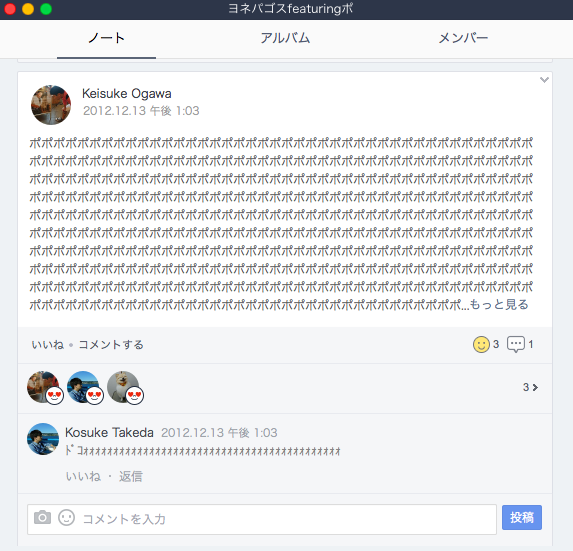
\includegraphics[scale=0.35]{yonepa.png}
    \subcaption{ヨネパゴスfeatringポ}
  \end{minipage}
  \begin{minipage}{0.4\linewidth}
    \centering
    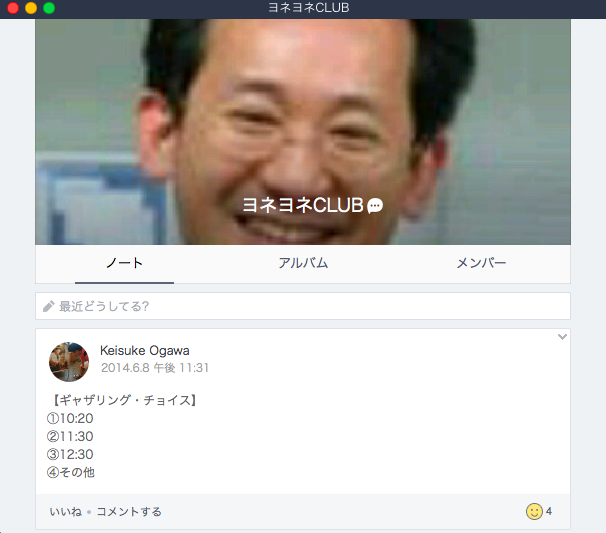
\includegraphics[scale=0.35]{yoneyone.png}
    \subcaption{ヨネヨネCLUB}
  \end{minipage}
  \caption{現存する唯一の最古の古墳たち}
  \label{yone}
 \end{figure}

まさに”これはひどい”の一言に尽きる。LINEという存在が普及し、ノートという機能の便利さにただただ感動していることが読み取れる。その中で、あの伝説の人間「オガワ・インティ・ライミ」が産声をあげたのもこの古墳である。その爆誕映像を図\ref{intira}に示す。\\

\begin{figure}[H]
  \centering
  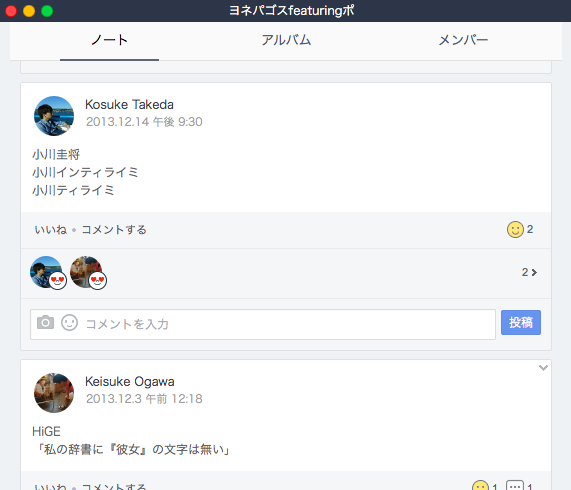
\includegraphics[clip,scale=0.5]{intira.png}
  \caption{オガワ・インティ・ライミ爆誕の瞬間。この時なんと2013年12月14日。偶然にも筆者がいまこの文章を執筆しているちょうど5年前である\sf (´\_ゝ`)笑}
\label{intira}
\end{figure}

そして時は流れ、これらの古墳たちを現代に甦らせ、高等技術専門学校により世界中に発信していこうという概念の下、生まれたのが「オガワ・インティ・ライミ公式ホームページ」である。
%---------------------------------------------------------------------------
\subsection{古舘プロジェクトという概念}

来たる2017年、オガワ・インティ・ライミの初代公式ホームページが突如爆誕した。そもそもオガワ・インティ・ライミとは何かすら、地球上の人間はその時点で知る由もないのだが、その後数秒で大スターに駆け上がるのである。そして、この公式ホームページを運営していたのはあの伝説の団体、古舘プロジェクト(Furutachi Project)である。この謎団体について以下に詳しく述べる。\\
 1984年7月1日、古舘伊知郎を始めとする将来を有望視された若き7人のブレーン達が、新時代の力となるべく立ち上った。各テレビ局等を辞め、自分達を表現する場を求めて独立、創設したのが古舘プロジェクトである。この団体の存在は、諸説あるが、図\ref{furutati_logo}のようなロゴを作成したとの報道もあるが、この真偽は不明である。\\
\begin{figure}[H]
  \centering
  
\includegraphics[clip,scale=0.4]{furutachi_logo.png}
  \caption{一説によると「株式会社古舘プロジェクト」と名乗っている偽団体もあるとか。そのロゴのセンスから、偽物であると言える。}
\label{furutachi_logo}
\end{figure}
わずか7人で始めた古舘プロジェクトも、今や社員総数70名(タレント、作家、ディレクター、スタイリスト等を含む)になり、マスコミ業界において非常に重要な地位を確立した。特にタレントと作家、ディレクターの質の高さにおいては、この業界屈指の頭脳集団である。社長をはじめ社員一同傲ることなく、マスコミにおけるベンチャー企業でありたいと、常に柔軟な姿勢で新しいものを追求している。\\
 古舘プロジェクトにとって最も大切な信念は「和」である。これは創設当時から変わらぬ理念である。この理念には、「人を思いやる心、感謝を忘れぬ心」が凝縮されたものである。決して傲ることなく、常に初心を胸に精進を積み重ねてきた結果として、今の古舘プロジェクトがある。今後も、この信念が変わることは無い。\\
 などと意味不明な供述をしているも模様。\\
 しかし、特筆すべきはそのメンバーである。図\ref{furutachi_member}をご覧いただきたい。重症患者「フルタチ」の他に、「ヨネスケ(ファンファン亭ヨネ助)」、「フルタチSFT」、「小川でやんす」が明記されているのである。ファンファン亭ヨネ助は紛れもなく重症患者であるが、「小川でやんす」はオガワ・インティ・ライミ氏が世を忍ぶ仮の姿であり、この存在を知っている人間は世界で約16億人とごくわずかであるため、非常に貴重な資料であると言える。したがって、この古舘プロジェクトという概念は、上記では偽団体と述べてしまったが、もはやそのような次元には存在しない、古舘という概念の概念を概念に概念で概念である。

\begin{figure}[H]
  \centering
  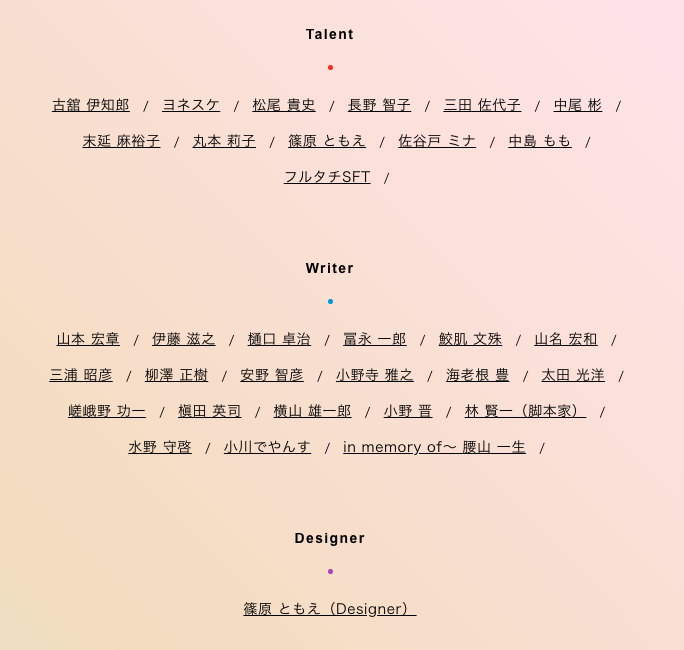
\includegraphics[clip,scale=0.4]{furutachi_member.png}
  \caption{果たしてこの全員が仕事をしているのか甚だ疑問である。}
\label{furutachi_member}
\end{figure}

%====================================
\section{初代公式ホームページ}
%====================================
 まあ、そんなこんなで、オガワ・インティ・ライミの初代公式HPが爆誕した。しかし、この初代公式ホームページは活動していないため、つい最近までその詳細は不明であった。しかし、本研究で様々な重症患者の努力によって開発された最新技術によってこの度約100000000000000光年だけ復元させることに成功した。図\ref{web1}にその時の様子を示す。現在はこのホームページが活動していないため、もはやこの画像はたいへん貴重なものである。\\
 ここで、この幻のホームページに記載されている超重要事項について、詳しく見ていく。\\

\begin{figure}[H]
  \centering
  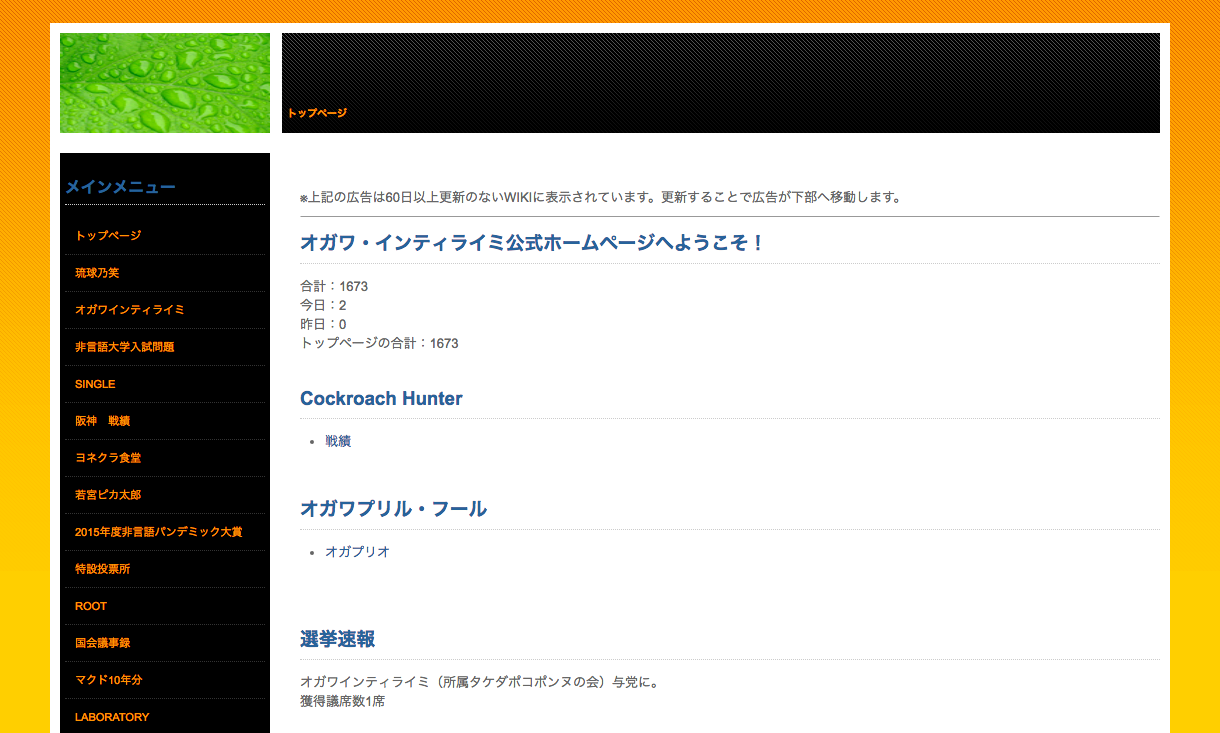
\includegraphics[clip,scale=0.35]{web1.png}
  \caption{編集しなさすぎてトップ画像がかき消えてるんやけど\sf (´\_ゝ`)笑}
\label{web1}
\end{figure}


\subsection{トップページ}
もはやトップページとその他になんの違いがあるのか甚だ疑問ではあるが、ある意味、衝撃的かつ革新的なトップページとなっている。各項目について、順次まあ適当に解説していく。\\
%\begin{enumerate}
\subsubsection{トップ画像}
 まずはじめに、トップ画像である(図\ref{web1_top})。これはひどいの一言で片付けたいところではあるが、詳しく見ていくことにする。まず謎の生命体が観測されるが、こいつは「D・ポマティ」という本物の人間であるが、ここに抜擢された理由として我々筆者である(ポ)、(マ)、(ティ)の融合体なのである。たしか、「ポマティ」でググったらこいつが出てきたとかんそんなん。他のデザインの由来は忘れた\sf (´\_ゝ`)笑\\
\begin{figure}[H]
  \centering
  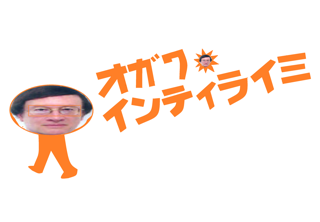
\includegraphics[clip,scale=0.6]{web1_top.png}
  \caption{That's 雑。この作画を担当したのはあの伝説のアブラガワ賞作家である又吉先生\index{またよしせんせい@又吉先生}である。}
\label{web1_top}
\end{figure}

\subsubsection{オガワ・インティライミ公式ホームページへようこそ!}
ここでは、図\ref{youkoso}のように、毎日の初代公式ホームページにアクセスした人数を集計している項目が載っている。基本的に、このホームページ内のページが変わる度に1カウントなので、来たついでに色々見ていると訪問者数がすごいことになる。したがって、その合計である「トップページの合計」はトップページを訪れた人数と一致しない。

\begin{figure}[H]
  \centering
  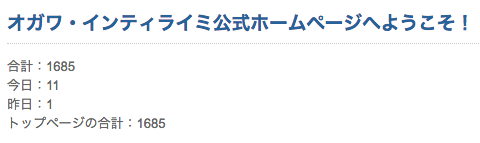
\includegraphics[clip,scale=0.5]{youkoso.png}
  \caption{このスクショの撮影するついでに色々見てたらクリック数が「11」になっただけであり、この日の正確な訪問者は筆者のみである。}
\label{youkoso}
\end{figure}

\subsubsection{Cockroach Hunter}
これは確か、G嫌いの(ポ)氏が、自らに打ち勝った功績を讃えるために、その戦場の記録を記そうとしたものである。しかし、蓋を開けてみると、この有様である(図\ref{cockroachhunter})。

\begin{figure}[H]
  \centering
  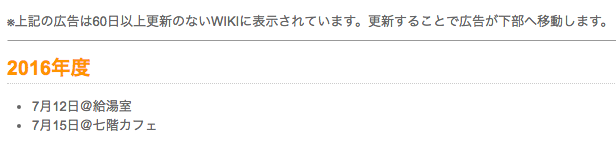
\includegraphics[clip,scale=0.5]{cockroachhunter.png}
  \caption{7階のカフェという概念}
\label{cockroachhunter}
\end{figure}

\subsubsection{オガワプリル・フール}
オガワ・インティ・ライミは嘘をつかないにもかかわらず、アンチがその判例を上げようと必死になっている世界である。図\ref{fool}のように、有る事無い事でっち上げもいいとこだが、そもそも「一覧」という概念について考えさせられるコーナーの一つである。

\begin{figure}[H]
  \centering
  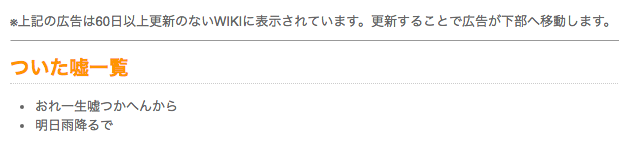
\includegraphics[clip,scale=0.5]{fool.png}
  \caption{そもそも「一生」なんて表現したことない気がする\sf (´\_ゝ`)笑}
\label{fool}
\end{figure}


\subsubsection{選挙速報}
オガワインティライミ(所属タケダポコポンヌの会)与党に。 \\
獲得議席数1席\\

\subsubsection{超速報}
\subsubsection{緊急小川速報 速報例}
この二つの速報たちは、突如現れた謎の存在である。しかし、下の「緊急小川速報 速報例」に関しては、内容が濃厚おばラーメンであり、もはや小川速報ではなくなっている始末である。しかも本文の「以下の表示はテストなので、大丈夫です」に関しては、何が大丈夫なのか。乞うご期待。
\begin{figure}[H]
  \centering
  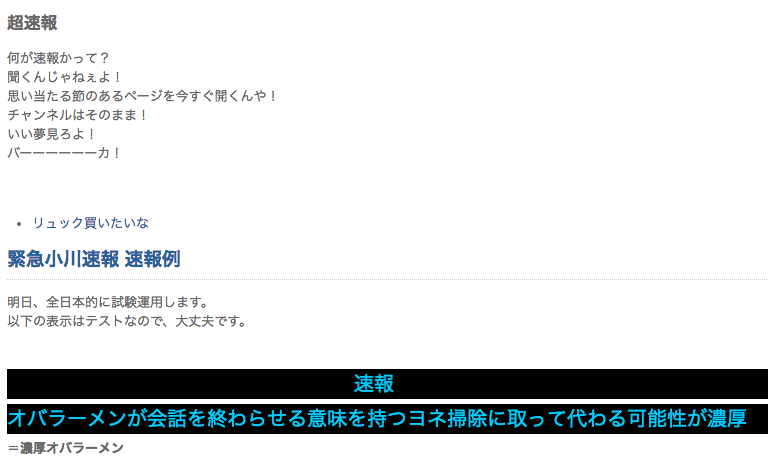
\includegraphics[clip,scale=0.5]{tyousokuhou.png}
  \caption{この謎の「リュック買いたいな」というリンクで飛ぶと、「このページへのアクセスは禁止されています。」と出る。}
\label{tyousokuhou}
\end{figure}

\subsubsection{ビッグバン}
宇宙の始まりであるとされているビッグバンは、実はその前にグバが存在していたという驚愕に事実が載っている。しかし、その過程と現在に至るまでの間に論理の飛躍があると思われており、現在調査中である。また図\ref{bigban}のように、その説明を(ポ)がしている矢先に琉球乃笑が緊急開店したことも推測される。

\begin{figure}[H]
  \centering
  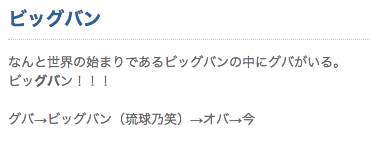
\includegraphics[clip,scale=0.6]{bigban.png}
  \caption{はたしてこのことについてグバ氏は知っているのか}
\label{bigban}
\end{figure}


\subsubsection{谷口ラーメン部発足}
その実態については不明であるが、少なくとも図\ref{enisi}のようにぐっさんがラーメンに必死になっていた記憶と記録は存在する。その時の名残であることが推測されるが、そのメニューとしての「LOG」ページを見ると図\ref{ramenlog}のような焼け野原であった。バラッッッッッ

\begin{figure}[H]
  \centering
  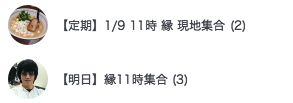
\includegraphics[clip,scale=0.6]{enisi.png}
  \caption{なお、【定期】メンバーはティライミとおば、【明日】はティライミと(ポ)、LINE中国語翻訳という異次元の組み合わせである。}
\label{enisi}
\end{figure}

\begin{figure}[H]
  \centering
  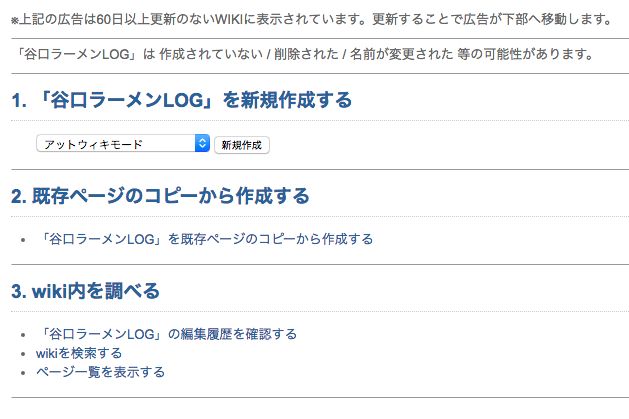
\includegraphics[clip,scale=0.5]{ramenlog.png}
  \caption{これはひどい。焼け野原もいいとこである。}
\label{ramenlog}
\end{figure}



\subsubsection{OGAZAP開店}
・ポの体重\\
\begin{figure}[H]
  \centering
  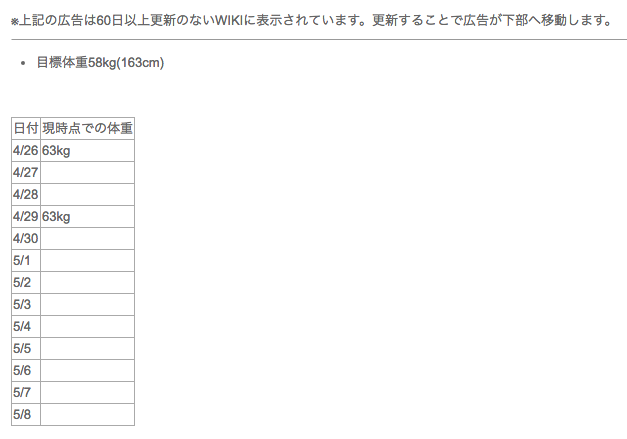
\includegraphics[clip,scale=0.5]{potaiju.png}
  \caption{ただでさえ少ない測定の上に、それらの測定結果である体重が同じという致命傷。}
\label{potaiju}
\end{figure}

・ティの体重\\
\begin{figure}[H]
  \centering
  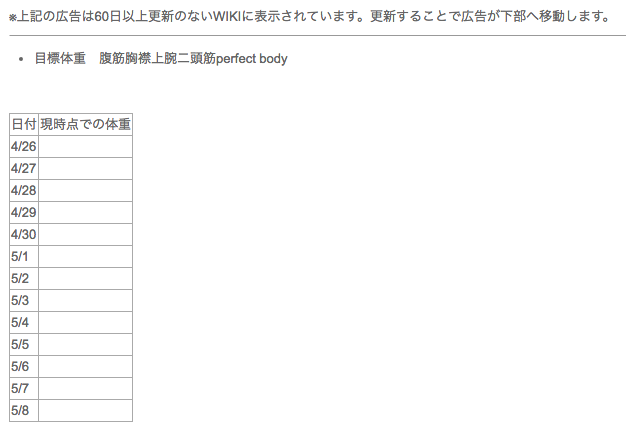
\includegraphics[clip,scale=0.5]{tetaiju.png}
  \caption{目標体重という概念}
\label{tetaiju}
\end{figure}


\subsubsection{谷口大学医学部発足}
稀代の天才オガワ、1000年に一度の鬼才グバヲが初代総長になり発足させた大学。 \\
医学部からはかの有名な重症患者たちも多数輩出されているとか、していないとか。\\

\begin{enumerate}
\item 入学案内・募集要項\\
いやまずはこれはひどい\sf (´\_ゝ`)笑\\

\begin{figure}[H]
  \centering
  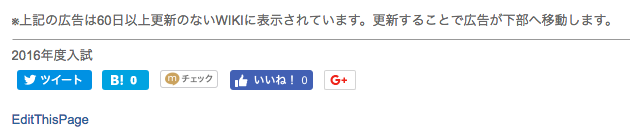
\includegraphics[clip,scale=0.5]{taniguti1.png}
  \caption{ばらっっっっっっっっっっっっっっっ}
\label{taniguti1}
\end{figure}

\item いままでの研究について\\
なぜ谷口氏の名前が、しかも先頭についているのか。\\
しかもよく見たら、谷口・オガワ脊髄「反応」の説明のはずが「著書である」という謎の締め方をしている。これはこれでこれはひどい。\\

\begin{figure}[H]
  \centering
  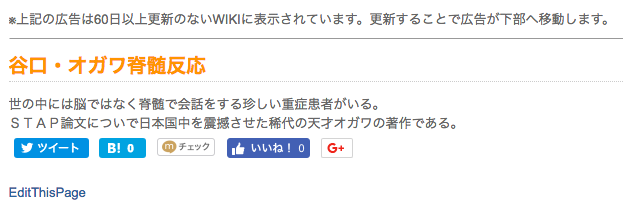
\includegraphics[clip,scale=0.5]{taniguti2.png}
  \caption{ばらっっっっっっっっっっっっっっっ}
\label{taniguti2}
\end{figure}


\item 用語解説\\
全く覚えていない\sf (´\_ゝ`)笑\\

\begin{figure}[H]
  \centering
  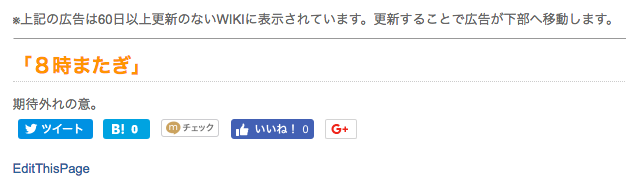
\includegraphics[clip,scale=0.5]{taniguti3.png}
  \caption{ばらっっっっっっっっっっっっっっっ}
\label{taniguti3}
\end{figure}

\end{enumerate}

\subsubsection{オバ国憲法(草案)}
独裁主義を保ちながら世界を揺るがす大帝国。\\
大叔母帝国憲法\\
\begin{enumerate}
\item 前 文\\ 
オバ国民は、正当に選挙された国会における代表者を通じて行動し、われらとわれらの子孫のために、諸国民との協和による成果と、わが国全土にわたつて自由のもたらす恵沢を確保し、政府の行為によつて再び戦争の惨禍が起ることのないやうにすることを決意し、ここに主権が国民に存することを宣言し、この憲法を確定する。そもそも国政は、国民の厳粛な信託によるものてあつて、その権威は国民に由来し、その権力は国民の代表者がこれを行使し、その福利は国民がこれを享受する。これは人類普遍の原理であり、この憲法は、かかる原理に基くものである。われらは、これに反する一切の憲法、法令及び詔勅を排除する。 \\
オバ国民は、恒久の平和を念願し、人間相互の関係を支配する崇高な理想を深く自覚するのであつて、平和を愛する諸国民の公正と信義に信頼して、われらの安全と生存を保持しようと決意した。われらは、平和を維持し、専制と隷従、圧迫と偏狭を地上から永遠に除去しようと努めてゐる国際社会において、名誉ある地位を占めたいと思ふ。われらは、全世界の国民が、ひとしく恐怖と欠乏から免かれ、平和のうちに生存する権利を有することを確認する。\\ 
われらは、いづれの国家も、自国のことのみに専念して他国を無視してはならないのであつて、政治道徳の法則は、普遍的なものであり、この法則に従ふことは、自国の主権を維持し、他国と対等関係に立たうとする各国の責務であると信ずる。\\
オバ国民は、国家の名誉にかけ、全力をあげてこの崇高な理想と目的を達成することを誓ふ。\\

\item 第1章 オ バ\\
第1条 オバは、オバ国の象徴でありオバ国民統合の象徴であつて、この地位は、主権の存するオバ国民の総意に基く。\\ 
第2条 バ位は、世襲のものであつて、国会の議決したリベルテ典範の定めるところにより、これを継承する。 \\
第3条 オバの国事に関するすべての行為には、内閣の助言と承認を必要とし、内閣が、その責任を負ふ。 \\
第4条 オバは、この憲法の定める国事に関する行為のみを行ひ、国政に関する権能を有しない。 \\
  2 オバは、法律の定めるところにより、その国事に関する行為を委任することができる。 \\
第5条 リベルテ典範の定めるところにより摂政を置くときは、摂政は、オバの名でその国事に関する行為を行ふ。この場合には、前条第一項の規定を準用する。 \\
第6条 オバは、国会の指名に基いて、グバ総理大臣を任命する。\\ 
  2 オバは、内閣の指名に基いて、最高裁判所の長たる裁判官を任命する。\\
第7条 オバは、内閣の助言と承認により、国民のために、左の国事に関する行為を行ふ。\\ 
一 憲法改正、法律、政令及び条約を公布すること。 \\
二 国会を召集すること。 \\
三 衆議院を解散すること。\\ 
四 国会議員の総選挙の施行を公示すること。\\ 
五 国務大臣及び法律の定めるその他の官吏の任免並びに全権委任状及び大使及び公使の信任状を認証すること。 \\
六 大赦、特赦、減刑、刑の執行の免除及び復権を認証すること。 \\
七 栄典を授与すること。 \\
八 批准書及び法律の定めるその他の外交文書を認証すること。\\ 
九 外国の大使及び公使を接受すること。 \\
十 儀式を行ふこと。 \\
第8条 リベルテに財産を譲り渡し、又はリベルテが、財産を譲り受け、若しくは賜与することは、国会の議決に基かなければならない。\\

\end{enumerate}

\subsubsection{LDH脱退騒動についてのお詫び}
拝啓、ありがとうございます。 \\
このたびはLDH所属のオガワインティライミが正式にLDHを脱退することが決まりました。 \\
それにつきまして「WOWOW(ウォウウォウ)」において緊急生放送することが決定しました。\\ 
1月18日午後10時から24時間緊急生放送「脱退してごめんね、ごめんね」を放送することが決定しました。\\ 
つきまして小川の謝罪会見を番組内で行うことが決定しました。 \\
ぜひご覧ください。\\
WOWWOWについて\\

\begin{figure}[H]
  \centering
  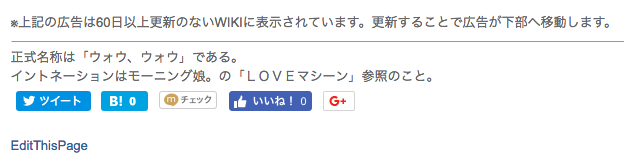
\includegraphics[clip,scale=0.5]{wowwow.png}
  \caption{wowwowという概念}
\label{wowwow}
\end{figure}

\subsubsection{自分用メモの更新}
もはや管理人が「自分」と言って出しゃばり、その速報を流すという暴挙である。その詳細は後ほどである。

\subsubsection{最新情報!!}
こういう速報は別にいいのだが、急なtwitterアカウントの爆誕であり、事実である。\\
なお開催の結果\\

\begin{figure}[H]
  \centering
  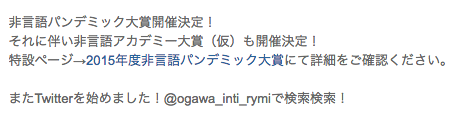
\includegraphics[clip,scale=0.5]{saisin.png}
  \caption{なんかホームページっぽい。}
\label{saisin}
\end{figure}


\subsubsection{挨拶}
いままでの速報欄が新しい順になっている、つまり時系列と逆の順番になっていることにここまで書いといて気づいた。まあいいや。\\
 公式ホームページとしては、はじめの挨拶というものは非常に重要である。いわば「顔」とも言える。仮にここで嘘をつくようなら、このホームページのタレント・アーティスト事態に信憑性が無くなるのである。果たして、以下に示す挨拶の内容は真実なのか、虚偽の申告なのかは管理人のみぞ知る。\\

\begin{figure}[H]
  \centering
  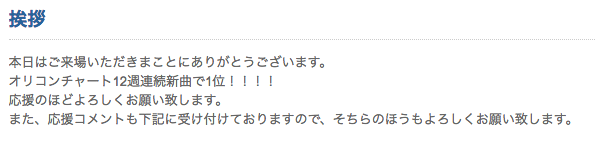
\includegraphics[clip,scale=0.5]{aisatu.png}
  \caption{来場という概念}
\label{aisatu}
\end{figure}

\subsubsection{オガワ・インティライミとは?}
\subsubsection{主にどのような活動をしているの?}
世界的に活躍している京都出身の男性シンガーソングライターです。 \\
様々な有名アーティストとの音楽活動、またその経験を活かし月に2回「古舘の館(旧 武道館)」でファンとの食事会を行っています。\\

\subsubsection{覚え書き}
「フェルマーの余白」という名ではあるが、もはやこれはひどいしか述べるべきことは存在しないのである。

\begin{figure}[H]
  \centering
  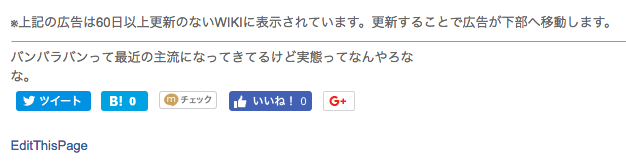
\includegraphics[clip,scale=0.5]{yohaku.png}
  \caption{The 焼け野原}
\label{yohaku}
\end{figure}


\subsubsection{訪問者数}
\subsubsection{人気投票}
\subsubsection{コメント欄}
これらは公式ホームページではよくある項目である。しかし、人気投票の立候補者に少々疑問が残るのである。\\
まずは「トゥ」という恐らく某教授ではあるのだが、ちょうど100票入っていることが怪しいのである。次に、その下のトゥースである。圧倒的な獲得票数13095票である。1票を投票するのに1秒かかるとして、3時間38分15秒かける計算になる。果たして本当に投票されたのかわからないが、今となってはこれも迷宮入である。\\
次に、コメント欄である。記念すべき一発目のコメント主が「古舘」という嘘である。もはやこの時点で意味がないのである。それからは大体が「やらせ」という表現で説明はつく。一方で、最新のコメント2つについては、真面目に関係者以外からの投稿であることが判明しており、その容疑者としてはグバ氏が挙げられているが、まだ犯人は捕まっていない。

\begin{figure}[H]
  \centering
  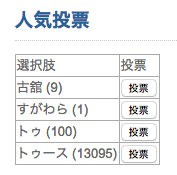
\includegraphics[clip,scale=0.6]{touhyou.png}
  \caption{ヒント:敬称略}
\label{touhyou}
\end{figure}

\begin{figure}[H]
  \centering
  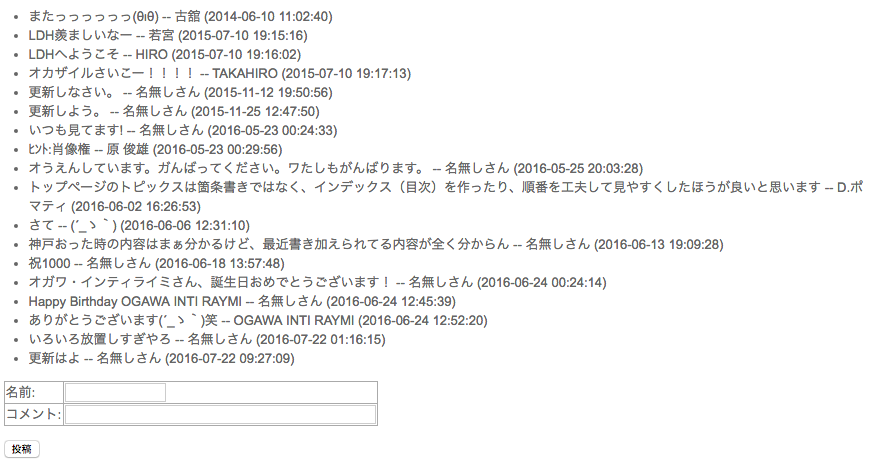
\includegraphics[clip,scale=0.5]{comment.png}
  \caption{実は真面目に藤田さんあたりが絡んでいるのでは、という推測も。}
\label{comment}
\end{figure}


%\end{enumerate}

\newpage
\subsection{メインメニュー}
はたしてメインとは。逆にメインではないのでは。基本的に、他に載ってないような項目に対してのみ詳細を述べる。

%\begin{enumerate}
\subsubsection{琉球乃笑}
後述。\par
\subsubsection{オガワインティライミ}
後述。\par
\subsubsection{非言語大学入試問題}
実質後述。なお、謎の表記があったため、以下に示す。

\begin{figure}[H]
  \centering
  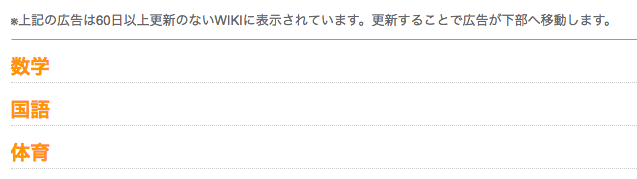
\includegraphics[clip,scale=0.6]{nyuusi1.png}
  \caption{いやこれはひどい。そもそも体育が入試にあるという驚愕の事実。}
\label{nyuusi1}
\end{figure}

\subsubsection{SINGLE}
後述。
\subsubsection{阪神 戦績}
急である。チョイスも全て謎である。ただなんとなく、言葉のチョイスとかがほんのりとぐっさんの匂いがする。

\begin{figure}[H]
  \centering
  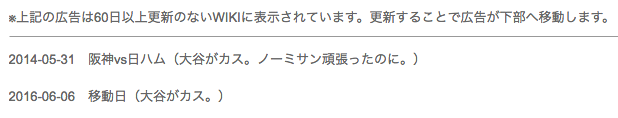
\includegraphics[clip,scale=0.6]{hansin.png}
  \caption{はたして何か長期間にわたって更新し続けた項目はあったのだろうか。}
\label{hansin}
\end{figure}

\subsubsection{ヨネクラ食堂}
筆者の記憶では、確かに「ヨネクラ食堂」というものは存在するのだが、初代公式ホームページ上には図\ref{yonekura}のような状態であった。

\begin{figure}[H]
  \centering
  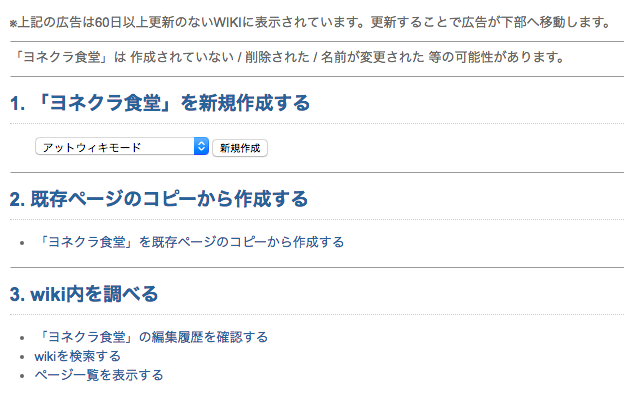
\includegraphics[clip,scale=0.5]{yonekura.png}
  \caption{いやこれもひどい。もはや状況すら理解できないのである。}
\label{yonekura}
\end{figure}

しかし、今一度ここで、伝説の「ヨネクラ食堂」を復活させる。最新の技術により復元されたものを図\ref{yonekura1}、\ref{yonekura2}に示す。図\ref{yonekura1}をみてもわかるように、メニューの全てが大好評であり、一つ一つが大手チェーン店の看板メニューを張れる実力があるものばかりである。おば直伝のおばカレーや、ヨネスケが解析的に物質量を定義したペヤング米森、オガワインティライミ公式ドリンクのカルピスなどがある。しかし、特に注目したいのは「とんかつ茶漬け」シリーズである。かつてオガワインティライミ氏と武田学長の間で一大ムーブメントを起こしたとんかつ茶漬け丼であるが、満を持してそのレシピを食堂のババアに尋ねたところ「うどんとかの出汁をかけてるだけ」と言われ、ばらぼんぬ古舘したという逸話も存在するものである。

\begin{figure}[H]
\centering
\begin{tabular}{cc}
\begin{minipage}{0.4\hsize}
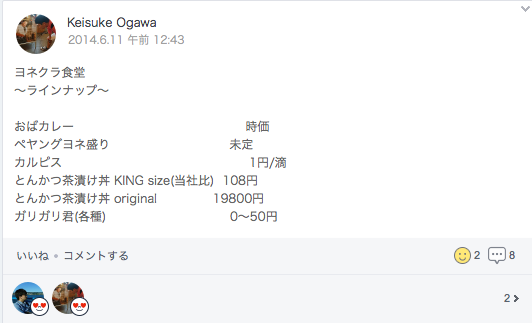
\includegraphics[scale=0.5,clip]{yonekura1.png}
\caption{時価という概念}
\label{yonekura1}
\end{minipage}

\begin{minipage}{0.4\hsize}
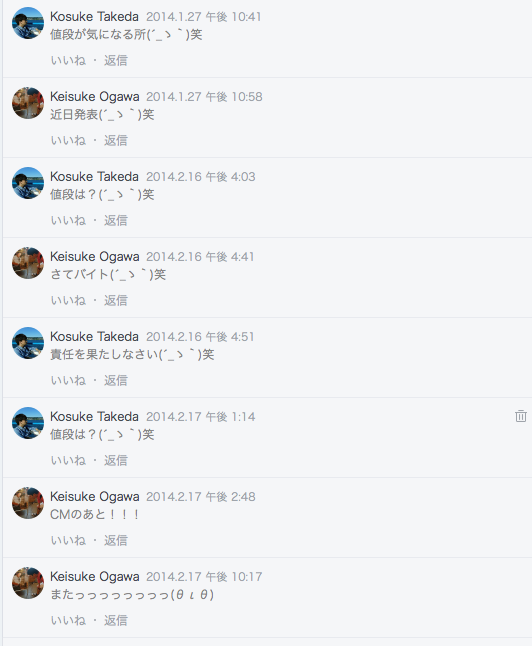
\includegraphics[scale=0.3,clip]{yonekura2.png}
\caption{ヨネクラ食堂には大勢のお客様が来店しているということが伺える。}
\label{yonekura2}
\end{minipage}
\end{tabular}
\end{figure}

\subsubsection{若宮ピカ太郎}
満を持して登場した往年のダークホース、若宮ピカ太郎。この人物の詳細について深く知ることができる項目かと思いきや、蓋を開けてみれば、図\ref{pika}の有り様である。

\begin{figure}[H]
  \centering
  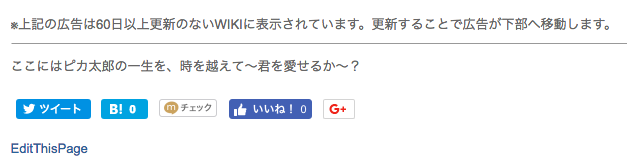
\includegraphics[clip,scale=0.5]{pika.png}
  \caption{もはや一発芸の領域である。}
\label{pika}
\end{figure}

\subsubsection{2015年度非言語パンデミック大賞}
 これは、その一年で蔓延した非言語の大賞を決めようという前代未聞の試みをしたものである。人間界では「流行語」という表現で通っているが、実際には「パンデミック」という表現が正しい。知らんけど。\\
 しかし、その実態は大きな謎に包まれている。まず、ノミネートがどのタイミングでなされたのか。そしてその選考委員は誰なのか。もはやこの大賞の価値はあるのか。と言うより、大賞はいつ決まるのか。2015年度以降の大賞は存在するのか、謎が謎を呼ぶと言っても過言である。\\
 ノミネート一覧を以下に示す。と言いたいところだが、なぜか初代公式ホームページには図\ref{nomine}のように表記されていた。

\begin{figure}[H]
  \centering
  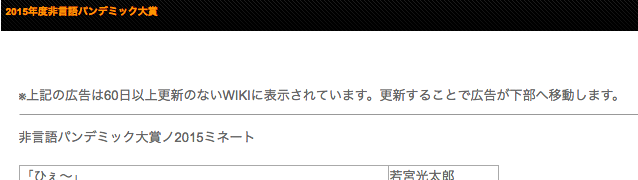
\includegraphics[clip,scale=0.5]{nomine.png}
  \caption{ノ2015ミネートという概念}
\label{nomine}
\end{figure}

まあそんなんことはさておき、ノミネート一覧を表\ref{nomine1}に示す。\\
注目したいのは「糞重/ポ」、「糞重爆撃祭り/ポ」である。このポこと(ポ)氏の正体が誰なのか、それによっては今後の選手生命に関わる大裁判に発展することが危惧される。また「Japan語/グ」を筆頭に「比叡山延暦寺/ポ」、「ピッカス where/ポ」、「解釈改憲/帝釈さん」、「決闘戦術\UTF{FF5E}Duel Tactics\UTF{FF5E}/グ」、「オバブクロ/バ」など、もはや使われた記憶すらないような非言語が飛び交っているのである。曖昧な選考基準や選考委員の存在だけでなく、この非言語パンデミック大賞自体の存在意義など、今後より詳細な研究を進めていくべき課題が多く存在するということが判明した。

\newpage
\begin{table}[htb]
\newcolumntype{C}{>{\centering}p{10em}}

	\begin{center}	\begin{tabular}{|c|c|} 
	\hline
「ひぇ\UTF{FF5E}」&若宮光太郎 \tabularnewline  \hline
「Japan語」&グ \tabularnewline  \hline
「今日は終わり」&ATM \tabularnewline  \hline
「糞重」&ポ \tabularnewline  \hline
「○○んや」&グ \tabularnewline  \hline
「比叡山延暦寺」&ポ \tabularnewline  \hline
「ピッカス」&ば \tabularnewline  \hline
「ピッカスwhere」&ポ \tabularnewline  \hline
「これは酷い」&ティ \tabularnewline  \hline
「マタキウム」&マタヨ \tabularnewline  \hline
「Fire Bird」&SEKAI NO OWARI \tabularnewline  \hline
「矢倉楓子」&グ \tabularnewline  \hline
「佐々木(窪田)」&ティ \tabularnewline  \hline
「(ピカ太郎=ピッカスということに対して)まぁカスやしな」&ば \tabularnewline  \hline
「クリロナ」&ティ \tabularnewline  \hline
「解釈改憲」&帝釋さん \tabularnewline  \hline
「決闘戦術\UTF{FF5E}Duel Tactics\UTF{FF5E}」&グ \tabularnewline  \hline
「おれ次第」&ば \tabularnewline  \hline
「カス、どこ行った?」&ば \tabularnewline  \hline
「マタペディア」&マタヨ \tabularnewline  \hline
「ぱーちくるふぃじっくす」&ば \tabularnewline  \hline
「マタハラ」&マタヨ \tabularnewline  \hline
「サレンダー」&ポ \tabularnewline  \hline
「糞重爆撃祭り」&ポ \tabularnewline  \hline
「クソキウム」&ポ \tabularnewline  \hline
「オバブクロ」&バ \tabularnewline  \hline
「コロチュウム」&ぐ \tabularnewline  \hline
「翔ちゃん」&ざわ \tabularnewline  \hline
「山元る」&やまげん \tabularnewline  \hline
「普通に」&若宮光太郎 \tabularnewline  \hline
	\end{tabular}
	\end{center}
	\caption{ノ2015ミネート}  
	\label{nomine1}
\end{table}

\newpage
\subsubsection{特設投票所}
これは、上記でノミネートされたカスどもに対し、この初代公式ホームページに訪れた強者たちに大賞を投票して決めてもらおうと試みたものである。図\ref{touhyou}、表\ref{kekka}にその惨状を示す。\\
注目したいのはその投票状況である。まず、ぱっと見で桁違いに投票数を稼いでいる項目がある。なんらかの権力が働いているとしか言えないような得票数である。そしてそれらは「ひぇ$\sim$」、「ぱーちくるふぃじっくす」、「山元る」といった錚々(そうそう)たる重症患者によってノミネートされたものであり、やはり何か法外な力がはたらいているということが完全に証明されたのである。知らんけど。\\
そもそも、この投票システムはワンクリックにつき1票であるため、例えば「ひぇ$\sim$」は200000001(2億1)クリックされたことになる。仮に、1秒で1クリックしたとして、6年4ヶ月以上もかかる。したがって、一人の力ではこの投票数を実現することは不可能であり、組織票、または投票システムの改変、または日本国民全員の協力を煽っているということになる。組織票は、重症患者という存在の特質から、考えにくい。これは組織票という概念が所詮人間の考える愚行であり、重症患者はそういう次元に生きていないからである。また、投票システムの改変は、重症患者はそんなことをしないと筆者が信じているため、これも違う。つまり、日本国民全員が協力し、投票した結果であると言える。やはり日本も捨てたもんじゃないということが言える。知らんけど。ばらあっっっっ。\par
てかよく見たら「これはひどい」が0票なのもおかしい気がする。めっちゃ使われてんのに\sf (´\_ゝ`)笑\\


\begin{figure}[H]
  \centering
  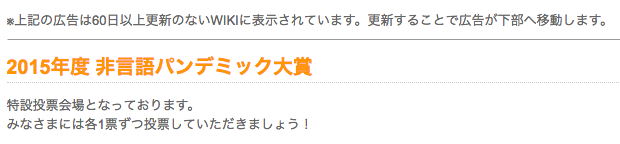
\includegraphics[clip,scale=0.5]{touhyou1.png}
  \caption{そもそも結果という概念}
\label{touhyou}
\end{figure}


\begin{table}%[h]
\newcolumntype{C}{>{\centering}p{10em}}

	\begin{center}	\begin{tabular}{|c|c|} 
	\hline
選択肢	&投票 \tabularnewline  \hline
ひぇ\UTF{FF5E} &(200000001) \tabularnewline  \hline
Japan語 &(1) \tabularnewline  \hline
今日は終わり& (2)\tabularnewline  \hline	
糞重 &(0)	\tabularnewline  \hline
○○んや& (0)\tabularnewline  \hline
比叡山延暦寺& (1)\tabularnewline  \hline
ピッカス &(0)\tabularnewline  \hline
ピッカスwhere &(0)\tabularnewline  \hline
これはひどい &(0)\tabularnewline  \hline
マタキウム &(0) \tabularnewline  \hline
Fire Bird &(1) \tabularnewline  \hline
矢倉楓子 &(0)\tabularnewline  \hline
佐々木[窪田]& (1)\tabularnewline  \hline
まぁカスやしな& (0)\tabularnewline  \hline
クリロナ &(0)\tabularnewline  \hline
解釈改憲 &(0)\tabularnewline  \hline
決闘戦術\UTF{FF5E}Duel Tactics\UTF{FF5E} &(0)\tabularnewline  \hline
おれ次第 &(1)\tabularnewline  \hline
カス、どこいった? &(0)\tabularnewline  \hline
マタペディア &(0)\tabularnewline  \hline
ぱーちくるふぃじっくす&[1.0E+47](4)\tabularnewline  \hline	
マタハラ &(1)\tabularnewline  \hline
サレンダー& (0)\tabularnewline  \hline	
糞重爆撃祭り& (0)\tabularnewline  \hline
クソキウム &(0)\tabularnewline  \hline
オバブクロ &(1) \tabularnewline  \hline
コロチュウム& (0) \tabularnewline  \hline
翔ちゃん &(0) \tabularnewline  \hline
山元る &(400001)\tabularnewline  \hline
普通に &(0) \tabularnewline  \hline
	\end{tabular}
	\end{center}
	\caption{オバブクロとは}  
	\label{kekka}
\end{table}

\newpage
\subsubsection{ROOT}
まずはこちらをご覧いただきたい。\\

\begin{figure}[H]
  \centering
  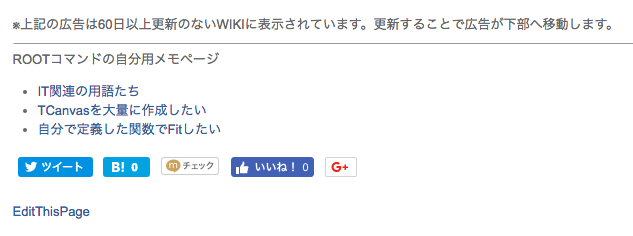
\includegraphics[clip,scale=0.5]{root.png}
  \caption{ヒント:メインメニュー}
\label{root}
\end{figure}

読んで字のごとく、ROOTのメモページである。\\
ROOT(ルート)は、CERNによって開発が行われている、データ解析環境および関連するライブラリ群である。グラフ作成のみならず、ヒストグラムの操作、4元ベクトルの扱い、実験データの可視化など、高エネルギー物理学の研究に不可欠な要素が組み込まれている。開発当初は素粒子実験のデータ解析用ソフトウェアとして構築されたが、近年では高エネルギー宇宙物理学や高エネルギー天文学といった分野でも使用されている。\\
まず、そのメモがこの初代公式ホームページに存在するのもおかしい上に、おそらくこのホームページの管理人の「自分用」のメモページなのである。この公私混同っぷりは、人間界ならば重罪ともとれるが、あくまで重症患者の概念においては通常運転なのである。\\
一方で、これらの蓋を開けてみると、新たな世界が広がっている。以下に、各項目を見ていく。ちなみにその価値があるかどうかの議論については今回は省略する。\\


\begin{itemize}
\item IT関連の用語たち
\begin{figure}[H]
  \centering
  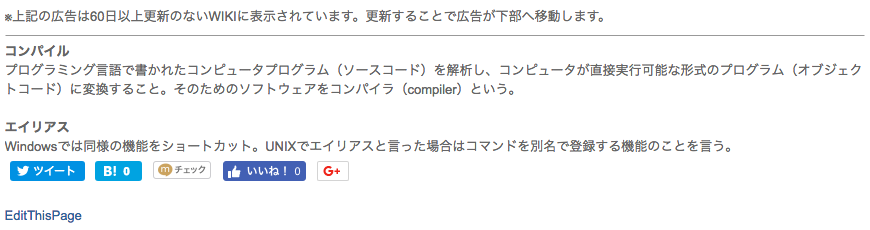
\includegraphics[clip,scale=0.4]{root1.png}
  \caption{そうなんかもしれんけども\sf (´\_ゝ`)笑}
\label{root1}
\end{figure}

\newpage
\item TCanvasを大量に作成したい

\begin{figure}[H]
  \centering
  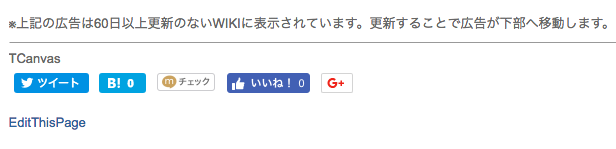
\includegraphics[clip,scale=0.6]{root2.png}
  \caption{いやこれはひどい\sf (´\_ゝ`)笑}
\label{root2}
\end{figure}

\item 自分で定義した関数でFitしたい

\begin{figure}[H]
  \centering
  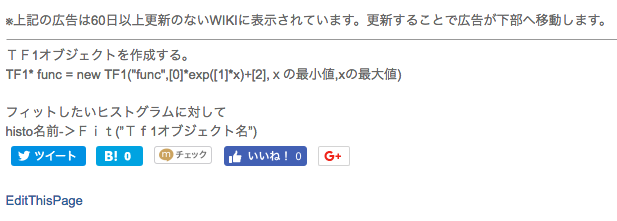
\includegraphics[clip,scale=0.6]{root3.png}
  \caption{これはオガワインティライミ氏が非常にお世話になったという噂も\sf (´\_ゝ`)笑}
\label{root3}
\end{figure}

\end{itemize}

\subsubsection{国会議事録}
これはおそらく、重症患者初の内閣総理大臣になったという噂のグバ総理大臣と、野党代表である(ポ)氏並びにオバ氏と、オガワインティライミ氏による国会答弁の議事録である。日々、壮絶な議論が繰り広げられており、その一部をご覧いただきたい。\\

{\bf2016/01/27}\\
ポ「emacs が応答してくれへん」 \\
グ「それはReflection Xが悪い」 \\
ポ「え、そうなん?」 \\
{\Large {\bf グ「そんなことはない」}}\\
 \\
{\bf2016/01/29} \\
グ「高松商業は猿みたいな高校やな」\\ 
ティ「猿とは」 \\
{\Large {\bf グ「知らんけど」}}\\
 \\
{\bf2016/01/30} \\
グ「ATMさんがこの研究室におれるのもあの人(Y山さん)のおかげらしいで」\\
ティ「え、そうなん?」 \\
{\Large {\bf グ「知らんけど」}}\\
 \\
{\bf2016/02/02}\\ 
グ「今日は雨って言ったろう!」\\ 
皆「え、そうなん?」 \\
{\Large {\bf グ「え、適当」}}\\
 \\
{\bf2016/02/03}\\ 
ポ「肉まんの”まん”ってなんなん?」\\ 
グ「まんじゅうの”まん”」\\
ポ「え、そうなん?」\\
{\Large {\bf グ「知らん」}}\\
 \\
{\bf2016/06/06}\\ 
ティ「旅立ちの日に聞いたらクリーンルーム思い出す」\\
ポ「い\UTF{FF5E}い日、旅立ち\UTF{FF5E}♪」\\
{\Large {\bf グ「あぁ、変なおばさんが歌ってるやつ」}}\\
 \\

\subsubsection{マクド10年分}
後述。

\subsubsection{LABORATORY}
一見、有意義な情報が盛りだくさんなのかと思いきや、ただのメモである。この仕業もこの初代公式ホームページの管理人である(ポ)氏であり、もはや上記の「ROOT」となんの違いがあるかは不明であり、今後より詳細な研究が必要である。一応、その項目だけ抜粋し、図\ref{labo}と共に以下に示す。

\begin{figure}[H]
  \centering
  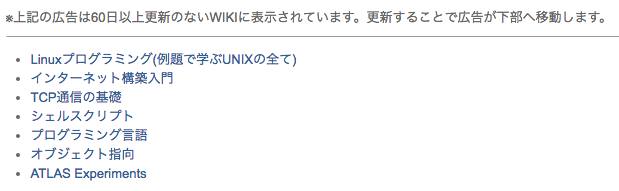
\includegraphics[clip,scale=0.6]{labo.png}
  \caption{地味に何言ってるかわからへんから本格的に触れられないという}
\label{labo}
\end{figure}


・Linuxプログラミング(例題で学ぶUNIXの全て)\\
 ・バッファリングの基礎\\
 ・セマフォ\\
 ・共有メモリ\\
 ・メッセージキュー\\
 ・3章 ファイルの操作\\
 ・8章 開発ツール\\
 ・13章 ソケット\\

・インターネット構築入門\\
 ・1章 TCP/IPとは\\

・TCP通信の基礎\\
 ・TCP通信の流れ\\

・シェルスクリプト\\
 ・シェル\\
 ・シェルスクリプト\\
 ・Bourneシェルスクリプト\\
 ・expr\\

・プログラミング言語\\
 ・多重継承\\
 ・入出力ストリーム\\

・オブジェクト指向\\
 ・用語説明\\
 ・オブジェクト指向開発の手順\\

・ATLAS Experiments\\
 ・略語一覧\\
 ・トリガーシステム\\
 ・ROD\\

\subsubsection{ATM road to heaven}
後述。
\subsubsection{外部リンク}
公式ホームページにありがちな項目ではあるが、ここに明記されているのは下記のようなものである。\\
http://www.nananaoto.com/\\
ナオトインティライミの公式ホームページである。これ以上のコメントは控えさせていただく。\\
ちなみに、この公式ホームページを見てみると、図\ref{naoto}のようになっている。完全なるバラボタンである。\\

\begin{figure}[H]
  \centering
  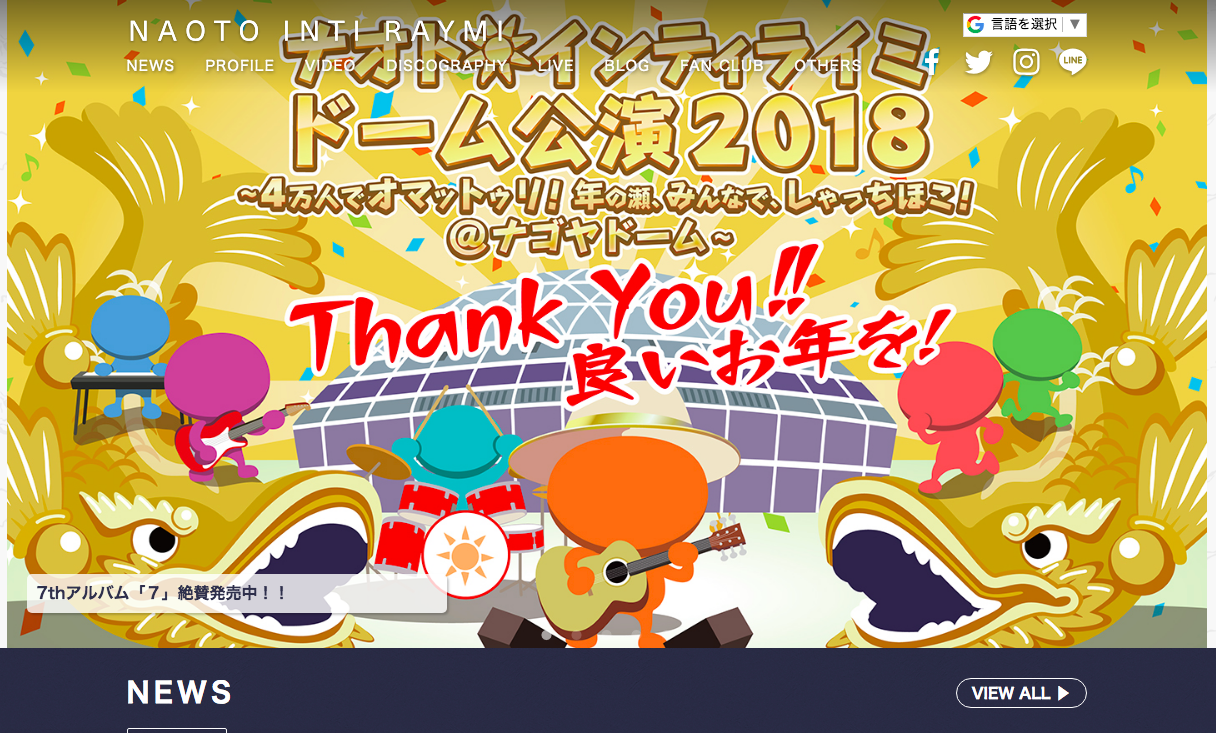
\includegraphics[clip,scale=0.2]{naoto.png}
  \caption{このスクショを取ったのは2019年の初めである。これはひどい。この一年は何もしないつもりだろうか。}
\label{naoto}
\end{figure}

%\end{enumerate}		

\subsection{その他}
以下の項目については、初代公式ホームページにも存在するが、その詳細については次節で述べる。\\
まあ、要するに次節がメイン的な。
\begin{enumerate}
\item オバ特殊警察失言集
\item グバ総理失言集
\item 会話のオガッショルド
\item 2015年度非言語パンデミック大賞
\item ある程度速報
\item Road to World War III
\item マクド10年分
\item バラク・オガワ就任演説
\item ATM road to heaven
\item SINGLE
\end{enumerate}


\newpage
%=========================================
\section{初代OFFICIAL WEB PAGE}
%=========================================
ヒント:二代目\sf (´\_ゝ`) \\
それはさておき、この初代OFFICIAL WEB PAGEが爆誕した経緯を述べる。事件が起こったのは2018年である。あの伝説の管理人(ポ)氏によって企画された、オガワ・インティ・ライミ氏の誕生日を祝した記念すべき概念である。基本的には初代公式ホームページと同じような概念の元で作成されたものであるが、そのクオリティは一目瞭然である。まずはそのトップ画をご覧いただきたい (図\ref{web2_top})。\\

\begin{figure}[H]
  \centering
  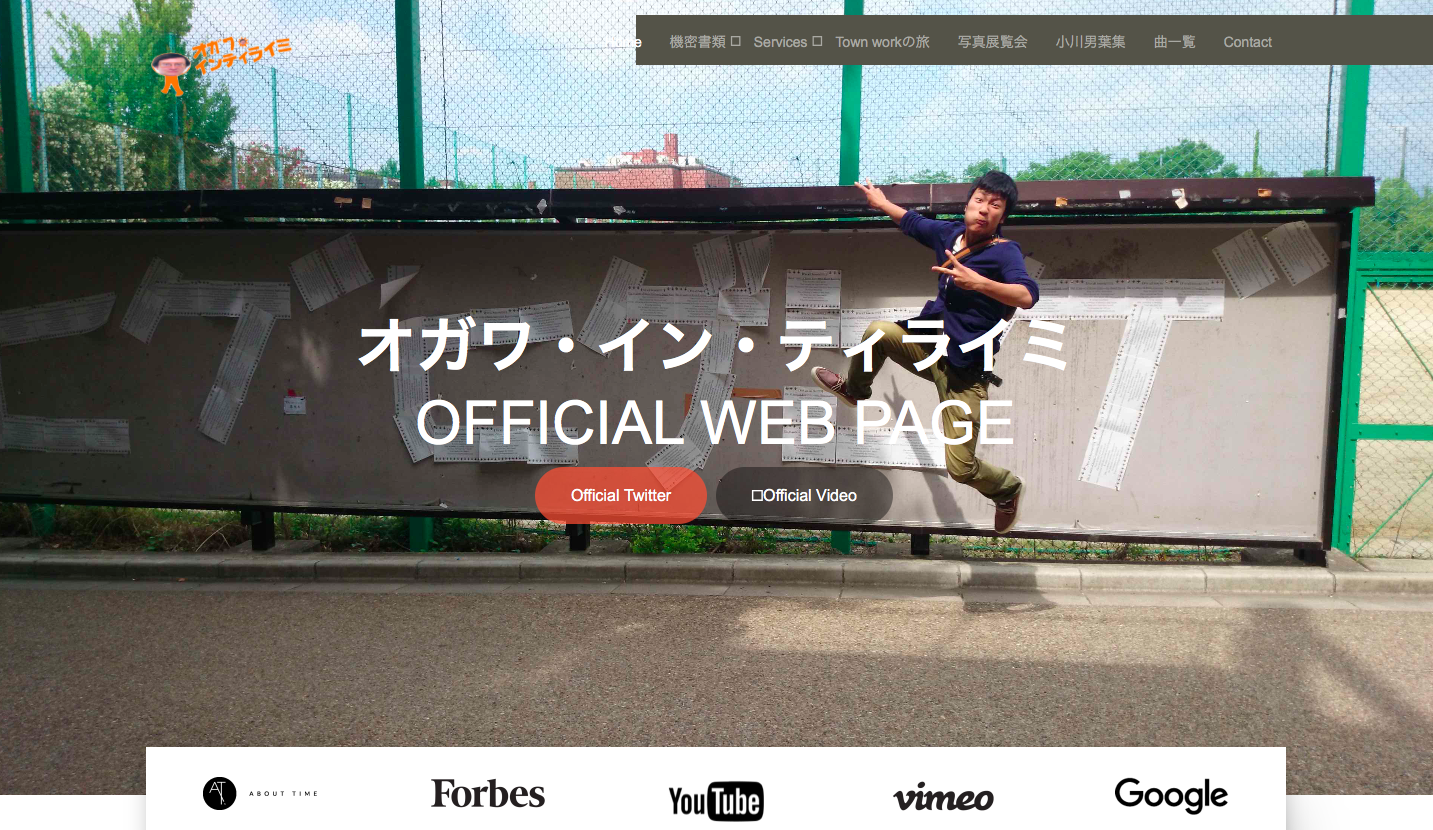
\includegraphics[clip,scale=0.3]{web2_top.png}
  \caption{このころは暇やった\sf (´\_ゝ`)笑}
\label{web2_top}
\end{figure}

非常にOFFICIAL WEB PAGEという概念と一致する、素晴らしい作品である。実際に、いわゆる誕生日プレゼントという形で受け取ったオガワインティライミ氏はそのクオリティの高さに非常に驚いたそう。と言うより「どれほど面白いんだろう」という期待をしていたのだが、あまりにもクオリティが高すぎて逆に笑ってしまうという事態になったそう。\\
ちなみにこのトップ画の写真は、おそらくB4の頃の大学院のオープンキャンパスとして某京都の大学に降臨した時の奇跡の瞬間を撮ったものである。なんでのない大学の掲示板に貼ってあった紙が「ヒゲ」の形をしていたのである。しかも複数あり「ヒゲヒゲヒゲ」となっていた。もはやこの時点でこの某京都大学がヒゲに汚染されているということが推測される。ちなみに\ref{hagehage}節で述べているハゲもこの某京都大学出身である。そしてオガワインティライミ氏や(ポ)氏、又吉先生\index{またよしせんせい@又吉先生}が存在していた伝説の研究所の支配下にいるヒゲの実の弟も某京都大学出身だとか。もはやこの場所も概念になりつつあるということが推測される。ぼん。\\
次に、この初代OFFICIAL WEB PAGEを構成する項目について解説する。大きく分けて「公式アカウント」、「トップページ」、「メインメニュー」の3つの項目がある。以下に、各項目について詳しく見ていくことにする。\\

%------------------------------------------------
\section{公式アカウント}
%------------------------------------------------
図\ref{web2_top}の中央にもあるように、このオガワインティライミ公式OFFICIAL WEB PAGEの他にオガワインティライミの公式による運営アカウントが存在する。その一つが公式Twitterアカウントである。図\ref{web2_top}の左の「Official Twitter」をクリックすると図\ref{twitter}のような公式アカウントのページに飛ぶ。これについて詳しく示したものを図\ref{twitter_t}に示す。\\


\begin{figure}[H]
  \centering
  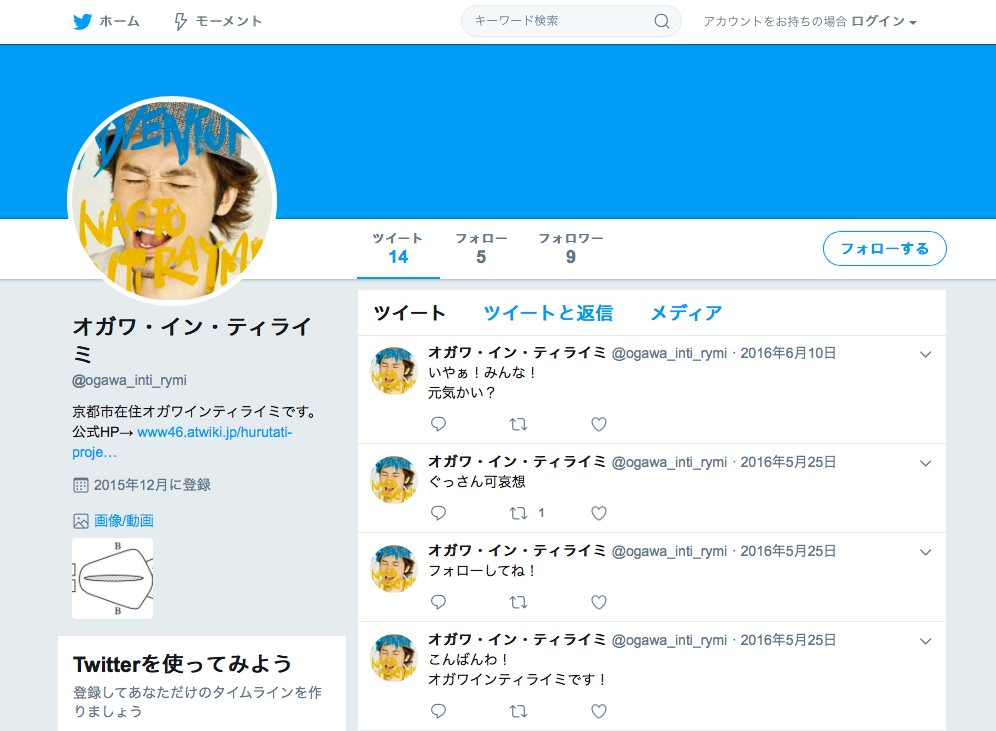
\includegraphics[clip,scale=0.3]{twitter.png}
  \caption{オガワ・インティ・ライミ公式twitterアカウント。}
\label{twitter}
\end{figure}

\begin{figure}[H]
  \centering
  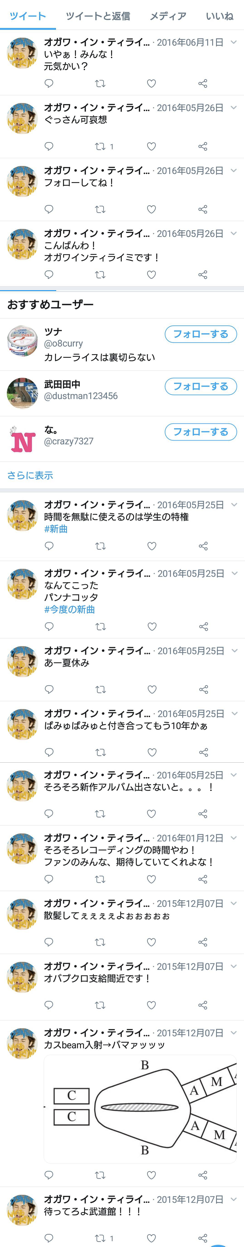
\includegraphics[clip,scale=1]{twitter_t.png}
  \caption{オガワ・インティ・ライミ公式twitterアカウントの詳細}
\label{twitter_t}
\end{figure}

一説によると、この「おすすめユーザー」に示されている「ツナ」はあの伝説の重症患者「おばツナ」ではないかと言われており、また「武田田中」はあの伝説のカス重症患者「さわだ」であると言われている。本研究を行っている中でさわだ氏は「適当なアカウント名を考えるときはだいたい武田田中を使う。理由はなんとなく」と述べている。もはやこれはさわだ氏が武田学長の支配下であり、それはすなわちれっきとした重症患者であるということが推測される。ひえ。\\
また、このオガワ・インティ・ライミの公式アカウントを運営している人物は謎に包まれている。しかしながら、2016年1月12日のツイートを注目していただきたい(図\ref{twitter_oba})。これを見る限り、いままで標準語を使っていたのにもかかわらず、突如関西弁を使い出したのである。これは管理人の正体が関西人であるという決定的な証拠である。果たしてこの管理人の正体は誰なのか、そもそも人間なのか、重症患者なのか、今後さらなる調査が期待される。\\
 さらに、ツイート頻度も問題の一つである。図\ref{twitter}に示される通り、まずツイート数が少ない。この時点でその活動の実態が怪しいのである。そして各々のツイート数を細かく見てみると表\ref{twitter_n}の通りである。全部で14ツイートという少なさに加えて、日にすると5日分のツイートしかしていないのである。果たしてこの公式アカウントの実態はいかに。ボンッッッッッッ\\
 次に、「Official Twitter」の右隣に「Official Video」が存在する。これをクリックするとYouTubeのとあるサイトに飛ぶ。一見、このオガワインティライミの公式チャンネルの公式動画かと思いきや、違うのである。その正体は「Dream Ami / トライ・エヴリシング (Dream Ami version) 」である。これはひどいのである(図\ref{try})。\\
 そもそも「トライ・エヴリシング」(Try Everything)は、2016年のディズニーのアニメ映画『ズートピア』の主題歌。オリジナル版ではシャキーラ、日本語吹替版ではDream Amiによって歌唱された。この日本語版は、Dream Amiの2ndシングル(サントラ版とは別バージョン[4])。2016年4月20日にrhythm zoneから発売された。トム・マクドゥーガル(ミュージック・スーパーバイザー)から高い評価を得て日本語版主題歌の起用[5]となった。\\


\begin{figure}[H]
  \centering
  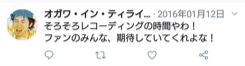
\includegraphics[clip,scale=1.7]{twitter_oba.png}
  \caption{オガワ・インティ・ライミ公式twitterアカウントによる疑惑のツイート。果たしてその正体とは。}
\label{twitter_oba}
\end{figure}

\begin{table}[htb]
\newcolumntype{C}{>{\centering}p{10em}}

	\begin{center}	\begin{tabular}{|c|c|} 
	\hline
ツイート日&ツイート回数 \tabularnewline  \hline
2015年12月07日&4 \tabularnewline  \hline
2016年01月12日&1 \tabularnewline  \hline
2016年05月25日&5 \tabularnewline  \hline
2016年05月26日&3 \tabularnewline  \hline
2016年06月11日&1 \tabularnewline  \hline
	\end{tabular}
	\end{center}
	\caption{ツイート回数の分布}  
	\label{twitter_n}
\end{table}

\begin{figure}[H]
  \centering
  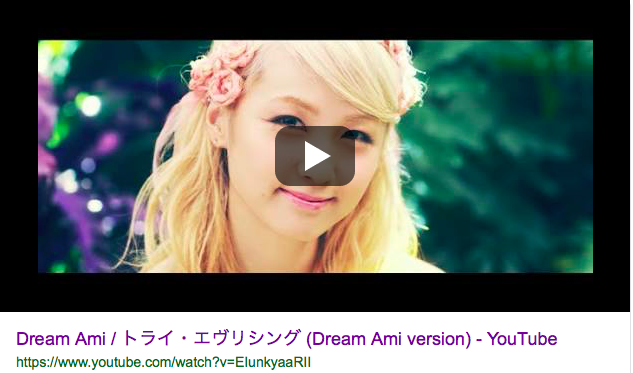
\includegraphics[clip,scale=0.5]{try.png}
  \caption{なんかソロデビューしたDream Ami的にはこれで結構注目された気がするけど、それでも一般的には誰やねんこれっていう。もう売れへんやろこいつまあまあな年齢やし。}
\label{try}
\end{figure}

\newpage
%------------------------------------------------
\subsection{トップページ}
%------------------------------------------------
%6069-7010-2631-8082-2223-6

燦然と輝くトップページには様々な項目が存在する。それらについてい以下に詳細を述べる。

%\begin{enumerate}
\subsubsection{オガワインティライミとは?}
世界的に活躍している京都出身の男性シンガーソングライターです。 2014年から活動を始め、徐々にその人気を伸ばしてきた彼が次に狙うのはノーベル平和賞。そんな彼の今後の活躍にも期待です!(図\ref{top_inti})\\

\begin{figure}[H]
  \centering
  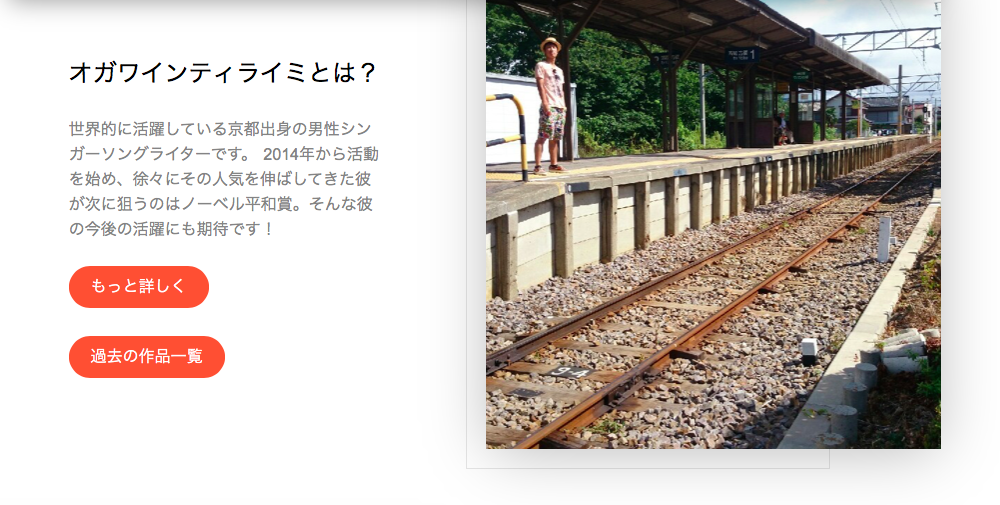
\includegraphics[clip,scale=0.3]{top_inti.png}
  \caption{なんか一丁前の画像を使用している。まあこれはよしとしよう。強いて言うなら懐かしの名古屋。}
\label{top_inti}
\end{figure}


{\bf 主にどのような活動をしているの?}
様々な有名アーティストとの音楽活動、またその経験を活かし月に2回「古舘の館(旧 武道館)」でファンとの食事会を行っています。\\
本日はご来場いただきまことにありがとうございます。 オリコンチャート12週連続新曲で1位!!!! 応援のほどよろしくお願い致します。 また、応援コメントも下記に受け付けておりますので、そちらのほうもよろしくお願い致します。\\
 \\
{\bf 事務所}\\
LDH\\
 \\
{\bf 経歴}\\
1993年6月24日、LDHからスカウトされ古舘プロジェクトを脱退したのち、6月25日にLDHに入団。\\
 \\
{\bf ライブ}\\
「古舘の館」で毎夏開催の恒例イベント。\\
D席:500円(10万席。立ち見)\\
C席:5万円(20万席保有。2階席奥。)\\
B席:15万円(15万席。2階席前方。)\\
A席:20万円(10万席。1階席後方。)\\
S席:50万円(6万席。1階席前方。)\\
SS席:100万円(1万席。最前列)\\
SSS席:200万円(5000席、最前列中央)\\
α席:500万円(100席。舞台袖)\\
β席:10億円(1部屋。ティライミの楽屋/窃盗等をはたらいた場合1兆円の罰金)\\
一日の興業収入、1040億円。\\
一週間連続公演。\\
さいごには5000万発(ちなみに日本最高の打ち上げ回数のPL花火大会は約1万発)の花火を打ち上げるのが恒例になっている。(この花火には50億円かかっている。)\\
D席での収入は京都市伏見区新町13丁目難民保護委員会へ寄付。\\

\subsubsection{過去の作品一覧}
{\large{\bf 2014年度}}\\
2014-05-29「Just crime/なんやねん、ゆかりって。」\\
 \ \ \ \ \ \ \ \ \ \ \ \ \ \ \ \ (B面:ゆかりのCMとタイアップ '14) \\
2014-05-29「またっっっっっっ($\theta$l$\theta$)」\\
 \ \ \ \ \ \ \ \ \ \ \ \ \ \ \ \ (ライブが終わるときの定番の曲) \\
2014-05-29「ぽんぬつゆ/オガワのティライミ節」 \\
2014-05-29「俺の道/J.J.」\\
 \ \ \ \ \ \ \ \ \ \ \ \ \ \ \ \ (B面は櫻井氏編曲) \\
2014-05-30「リアルescape/鯖祭り」\\
 \ \ \ \ \ \ \ \ \ \ \ \ \ \ \ \ (初回限定版はB面を北島三郎氏が歌っている) \\
2014-05-30「KE-A-NA/KE-A-NA(instrumental)」\\
 \ \ \ \ \ \ \ \ \ \ \ \ \ \ \ \ (琵琶湖花火大会のテーマソング) \\
2014-06-02「ポロポロは続くよ\UTF{FF5E}どこまでも\UTF{FF5E}/酒の河(arrange ver.)」 \\
2014-06-03「嗚呼、腹痛(リアル)/嗚呼、腹痛(dance ver.)」 \\
2014-06-03「Re:alistic escape/ウォシュレット」 \\
2014-06-06「もう嫌だ☆臭いだけでも☆吐けるのに。/ゲロゲロ天国」\\ 
2014-06-09「T.M.Re:volution/Just西川」 \\
2014-06-09「ゴッドギャザリング\UTF{FF5E}G.G.佐藤\UTF{FF5E}/ファンヨン亭ヨネ助」\\
 \ \ \ \ \ \ \ \ \ \ \ \ \ \ \ \ (A面はGG佐藤のテーマソング/B面は笑点のテーマソング) \\
2014-06-09「Happy Standridge/六甲颪」 \\
2014-06-19「SECOND DANCE type K /きよしの二の舞を踏むなんて。」\\ 
2014-06-20「御釜ノムコウ/床マァラッッッッッッッッ($\theta$l$\theta$)関数」 \\
2014-06-20「JJcrime 2014」 \\
2014-07-12「101回目のもう嫌だ/101回目のもう嫌だfeat.BUMP OF CHICKEN」\\
 \ \ \ \ \ \ \ \ \ \ \ \ \ \ \ \ (Mステで初披露) \\
2014-07-12「あの鐘をならすのはマラァッッッッッッッッッ/与作(カヴァーver.)」 \\
2014-07-13「任セロリ」\\
 \ \ \ \ \ \ \ \ \ \ \ \ \ \ \ \ (竹田プロデューサー作詞作曲編曲) \\
2014-07-13「Just 一般人people feat.浅沼亮介」 \\
2014-07-14「Google operator」\\
 \ \ \ \ \ \ \ \ \ \ \ \ \ \ \ \ (Google社の社歌)\\ 
2014-07-17「まさかの不可」\\
 \ \ \ \ \ \ \ \ \ \ \ \ \ \ \ \ (ドラマ『HiGE物語’09 物理数学篇』) \\
2014-07-22「Lezend of ハラスト/ハラストイレ」(H\&N記念ソング) \\
2014-07-22「あの和田を鳴らすのはアキ子/\\
 \ \ \ \ \ \ \ \ \ \ \ \ \ \ \ \ 日曜日よりの使者-歌いたいのはそこじゃないver-」 \\
2014-07-22「ハラストDiNNER(?)」 \\
2014-07-24「マエダマエダ」 \\
2014-07-25「world of soysource/Just醤油」\\ 
2014-07-25「僕の喉が追い付かない」\\
 \ \ \ \ \ \ \ \ \ \ \ \ \ \ \ \ (特典映像つき)\\ 
2014-07-31「Just 韓国の潤滑油/justバニラ」 \\
2014-08-04「私の頭の中のガイドブック/いきあたりおばったり」 \\
2014-08-04「ハラストラストの散乱問題」 \\
2014-08-04 「オバームクーヘンfeat.オダギリジョー/Just dirty\UTF{FF5E}鉄ウンコ\UTF{FF5E}」\\ 
2014-08-04 「ヨネ掃除」ヨッネヨネヨネ、ヨネ掃除 \\
2014-08-04「大回転発狂バズーカ\UTF{FF5E}ビッグカメラ遊戯王\UTF{FF5E}」\\ 
2014-09-07「THE 蟹」 \\
2014-10-22「Just 小畑feat.川端」\\ 
2014-10-23「Just HOME\UTF{FF5E}量子力学演習\UTF{FF5E}featケケポコ」\\ 
2014-12-02「Just fish\UTF{FF5E}鯖\UTF{FF5E}」 \\
2014-12-18「Justポール/ほぼうどん」\\
 \ \ \ \ \ \ \ \ \ \ \ \ \ \ \ \ (サバ後ろ食べ歩き)\\ 
2014-12-22「皮\UTF{FF5E}just moon light\UTF{FF5E}」 \\
2014-12-26「The End of Suspenders\UTF{FF5E}冬休みの訪れ\UTF{FF5E}」\\
 \\
{\large{\bf 2015年度}}\\
2015-01-08「complex conjugate 」\\
 \ \ \ \ \ \ \ \ \ \ \ \ \ \ \ \ (2014年流行語大賞受賞) \\
2015-01-08「just normalization\UTF{FF5E}寿命で死ねば良い\UTF{FF5E}」\\
 \ \ \ \ \ \ \ \ \ \ \ \ \ \ \ \ 発表は2014年12月、3代目JSBの大賞を剥奪したのち、レコード大賞受賞。\\
  \ \ \ \ \ \ \ \ \ \ \ \ \ \ \ \ これにより3代目JSBは解散の危機を迎えるがティライミの慈悲により免れる。\\
2015-01-23「カニ倶楽部feat.コブクロ」 \\
2015-01-29「Lezend liquid /カラシと揚げ出し豆腐」\\ 
2015-01-29「glass hopper/バッタバッタ」\\
 \ \ \ \ \ \ \ \ \ \ \ \ \ \ \ \ 妖怪ウォッチ、世の勝ち組が羽ばたくときに聞いといてもらいたい歌。\\
  \ \ \ \ \ \ \ \ \ \ \ \ \ \ \ \ 西田行政書士個人事務所公式応援歌\\
2015-01-29「n.a.n.a.c.o. feat3代目JSB\\
 \ \ \ \ \ \ \ \ \ \ \ \ \ \ \ \ /か、ら、し。feat 藤岡弘、$\times$2&モーニング娘。$\times$1」 \\
2015-02-02「ギラファノコギリクワガタfeat.aiko」\\
 \ \ \ \ \ \ \ \ \ \ \ \ \ \ \ \ (初回特典ムシキングのカード) \\
2015-02-02「Just New Year\UTF{FF5E}Natural science library\UTF{FF5E}」\\
 \ \ \ \ \ \ \ \ \ \ \ \ \ \ \ \ (生の餅の同梱版は3000枚限定)\\ 
2015-02-09「ゲートガーディアン坂本 feat. サスペンダーズ」\\
 \ \ \ \ \ \ \ \ \ \ \ \ \ \ \ \ (長期休暇前) \\
2015-04-12「オガワールド/08ワールド」 \\
2015-07-10「O.B.A.Crime/Just crime feat.O.B.A」\\
 \ \ \ \ \ \ \ \ \ \ \ \ \ \ \ \ (オバ新風降臨時原付事故故) \\
2015-09-06「小学生以下の方は何名いらっしゃいますか」 \\
2015-09-07「なんやねんこのクソヨンテふざけんなよ」\\
 \\
{\large{\bf 2016年度}}\\
2016-01-22「ねぎ溢れ/ねぎアフロ」\\
 \ \ \ \ \ \ \ \ \ \ \ \ \ \ \ \ (演歌風ラーメン風味。名島亭公式応援歌) \\
2016-01-25「それいけ腰パンマンfeat やなせたかし/深夜bash feat オバ」 \\
2016-01-25「ポグポグ feat.ポグポグ」 \\
2016-01-28「hot body bow」 \\
2016-02-03「ポグポグ2 feat.ポグポグ」\\ 
2016-04-04「胃袋という名のタッパーfeat.オバブクロ/ベルサイユのヘッ薔薇」 \\
2016-04-29「線源がノイズ宣言(ナオトインティライミlive ver.)」 \\
2016-05-20「バランバラン訪問」 \\
2016-05-20「小川のジレンマ/生えたいのに生えない」\\ 
2016-05-25「微粒子/雨が降りそうだから僕は傘を持っていく」\\
 \ \ \ \ \ \ \ \ \ \ \ \ \ \ \ \ (雨が降りそうやけど洗濯物がしたいという男心を歌ったパンクロックバラード)\\ 
2016-05-25「always autumn」\\
2016-05-26「QGP(quark-gluon plasma)」\\ 
2016-05-28「概念歌feat琉球乃笑」 \\
2016-05-30「平成の爆笑王/余剰次元反復横跳」\\ 
2016-05-31「朗読終了」 \\
2016-05-31「10Baller=1\$」\\ 
2016-05-31「ヤスオーラ/竹内康雄の憂鬱〜はぁ…僕専攻長なのになぁ…〜」 \\
2016-06-01「ヨネ大晦日」 \\
2016-06-01「ATM Road to Heaven/苦楽園」\\ 
2016-06-02「○○オペレーター作動」 \\
2016-06-08「私が研究室になったら/研究室は容量〜100人入っても大丈夫〜」 \\
2016-06-14「饒舌な爆笑トークで言語の壁を破壊する!crash the wall」 \\
2016-06-16「フラッシュコロキウム/消費税80‰」 \\
2016-06-17「KHD48」 \\
2016-06-18「オ・ヴァンゲン」\\ 
2016-06-18「もう若者なんていないfeat.愚馬朽曜威/ずっとおれfeat.おば」\\
 \ \ \ \ \ \ \ \ \ \ \ \ \ \ \ \ (バス停がずっと川端通り) \\
2016-06-29「第一次コラ画像」 \\
2016-07-03「全身タイツ」\\
 \ \ \ \ \ \ \ \ \ \ \ \ \ \ \ \ (サビ 心の全身タイツを着よう)\\
2016-07-08「20皿/食い過ぎオペレーター作動して頂いて構いません\\ 
 \ \ \ \ \ \ \ \ \ \ \ \ \ \ \ \ (それでは作動して頂きましょう、オガワインティライミさんで20皿、どうぞ)」\\ 
2016-07-10「僕はもう死にましぇ〜ん」\\
 \ \ \ \ \ \ \ \ \ \ \ \ \ \ \ \ (3回目の輪廻転生の主題歌) \\
2016-07-11「walking axilla」 \\
2016-07-11「惜しまれつつ開店feat.琉球乃笑」\\ 
2016-07-11「バランバランバランスボール/どうぞご自由に音頭」\\ 
2016-07-11「アバポンヌやあらへんで!!\\
 \ \ \ \ \ \ \ \ \ \ \ \ \ \ \ \ /第一億八千万回アバポンヌやあらへんで!!\\
  \ \ \ \ \ \ \ \ \ \ \ \ \ \ \ \ アバアバ オガワインティライミをつかめ!アバポンヌヶヶヶ〜〜〜!!!」 \\
2016-07-11「OGAPRIO/タイタニック」\\
 \ \ \ \ \ \ \ \ \ \ \ \ \ \ \ \ (タイタニックの主題歌、毎年4月1日のみダウンロード配信、\\
  \ \ \ \ \ \ \ \ \ \ \ \ \ \ \ \ 10年に一度、そのアルバムが発売される。現在2枚発売中。)\\

\subsubsection{小川男葉集}
古より伝わりし、小川家伝来の巻物。数々の編纂者が命を賭け、苦難を乗り越え、伝統を紡ぎ現在に伝わっています。 彼らの息遣いが聞こえてくる歴史的傑作箇条書本を特別に公開しています。\\
詳しくは\ref{manyomanyo}章を参照。\\

\begin{figure}[H]
  \centering
  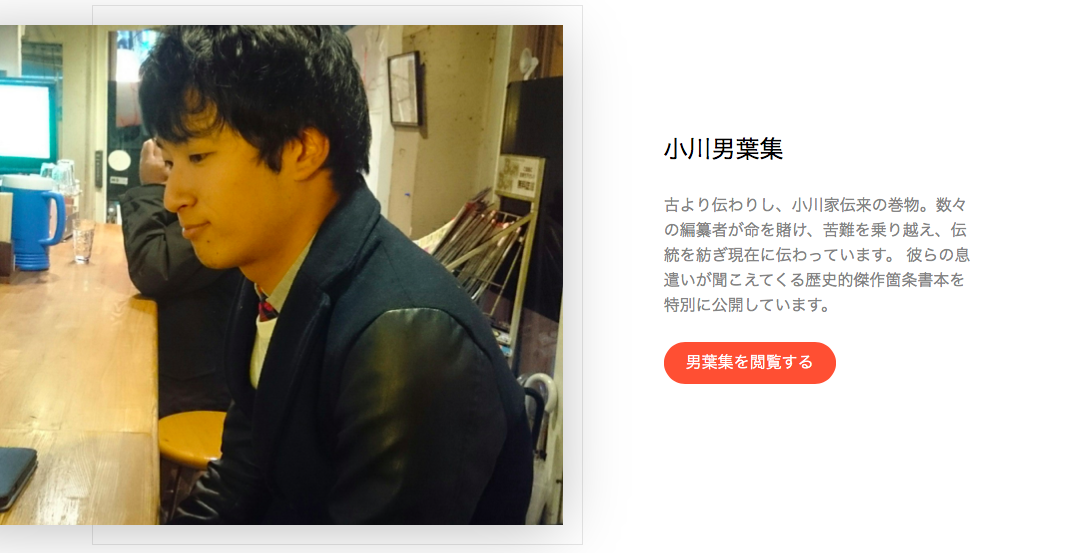
\includegraphics[clip,scale=0.3]{top_manyo.png}
  \caption{これはもう完全に絶望の瞬間の漢の画像である。この瞬間は完全に財布が紛失しているのである。完全に紛失である。}
\label{top_manyo}
\end{figure}

\subsubsection{概念論文}
6年に渡る研究の成果を携え、小川善沈丸、堂々の学生生活完結巨編。 全ては概念論文を執筆するために大学に入学し、大学院へと進学した。幾多の苦難を乗り越え、様々な人達と出会い、別れを繰り返してきた 男が魂を込めて筆を取った!!共同研究者には、又チチ大先生やアバポンヌ船長の生みの親である武田学長がおり、豪華な顔ぶれにも負けない 集大成。\\
しかし、まだ終わりではない。人生という名の概念論文はこれからも続く(図\ref{top_ronbun})。\\
 \\
という文章とともに、リンクを飛ぶと、図\ref{ronbun}のような概念が勃発する。

\begin{figure}[H]
  \centering
  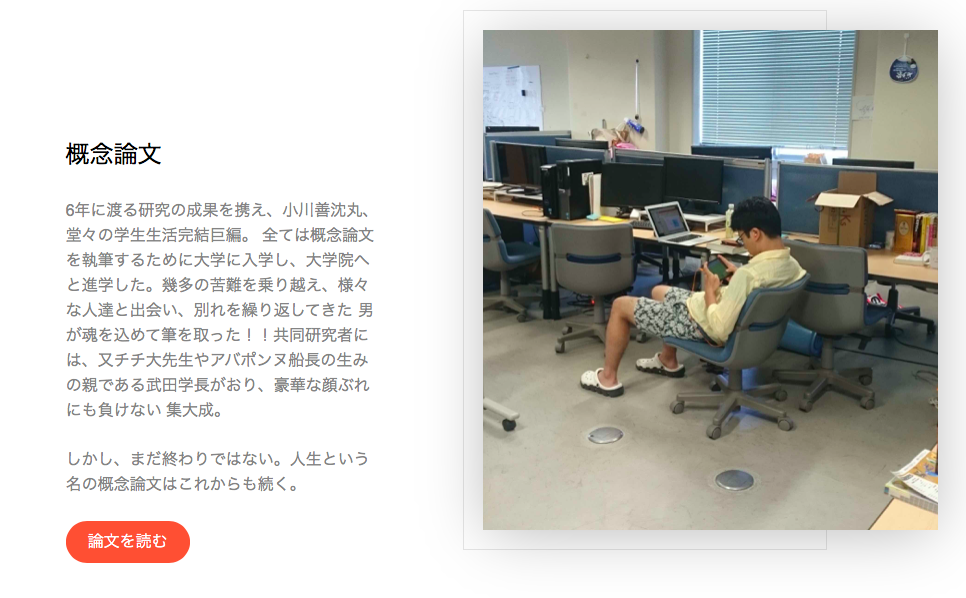
\includegraphics[clip,scale=0.3]{top_ronbun.png}
  \caption{伝説のアーティスト、オガワインティライミ氏が懸命に論文執筆をしている瞬間を撮影した貴重な画像である。まるでウイイレをしているかのような躍動感である。}
\label{top_ronbun}
\end{figure}

\begin{figure}[H]
  \centering
  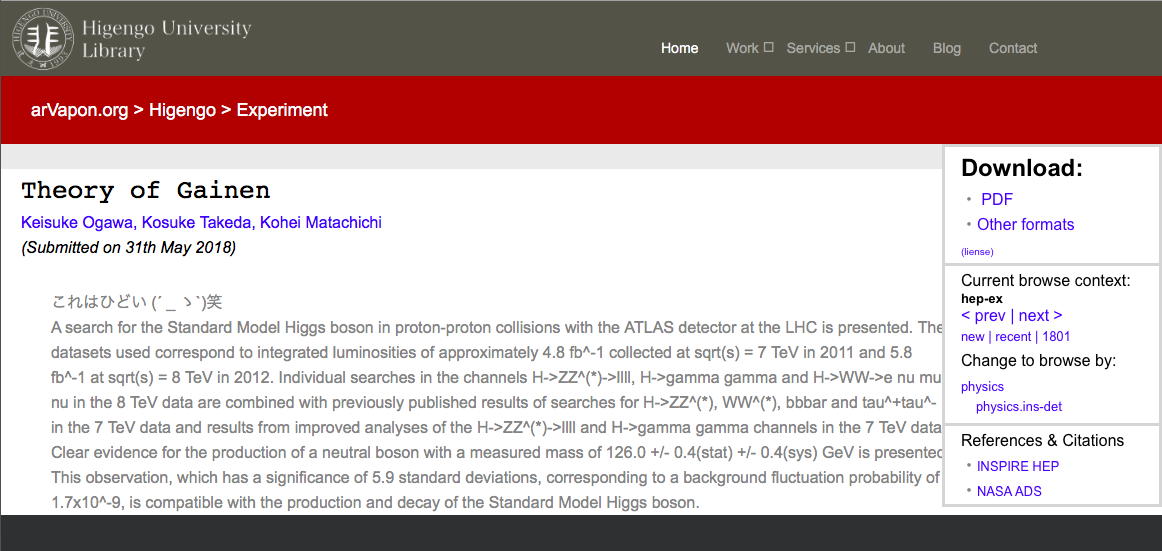
\includegraphics[clip,scale=0.3]{ronbun.png}
  \caption{本格的でシンプルにすごいと思った\sf (´\_ゝ`)笑}
\label{ronbun}
\end{figure}

\subsubsection{百ポ辞典}
2012年に全ては始まった。我々の心のふるさととも呼べる、国民的愛蔵書。 広辞苑を凌駕する精密さと緻密さと心強さを兼ね備えた次世代型辞典。 人類の英知が収録された、非常に高密度な言語録である。見逃さないでいただきたい。\\
現在、鋭意製作中。続報を待て。\\

\begin{figure}[H]
  \centering
  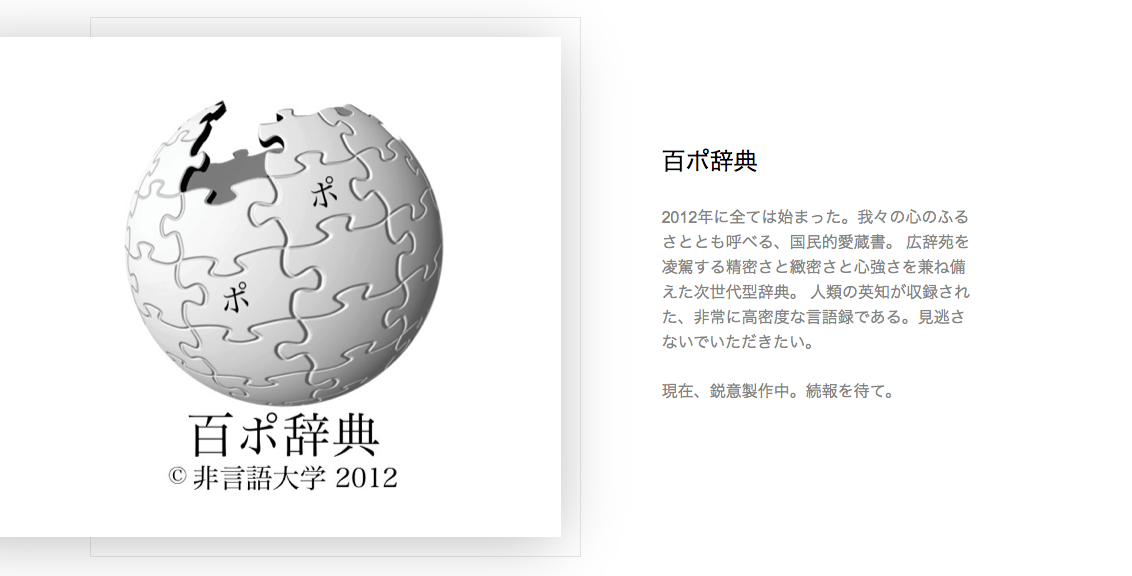
\includegraphics[clip,scale=0.3]{top_hyappo.png}
  \caption{}
\label{top_hyappo}
\end{figure}

と書いてあるが、本研究ではその百ポ辞典を復元することに成功した。以下に示す。\\
 \\
パゴーーーーーー\\
アバポンヌパゴリアス\\
{\bf 1-1.}\\
裸転体の法則\\
1-2\\
エスカルポ展開\\
1-3\\
不審者方程式\\
パセリ=ゲロ\\
1-3-1\\
パセリ=緑色\\
1-4\\
Fm展開定理(フェルマー)\\
1-5\\
企業社会論法\\
1-6\\
ソフトクリーム・菅原=爆笑\\
1-7\\
洋式=2和式\\
1-8\\
∇・(1/N)= θ\\
1-9 マイケル・ジャクソン現象\\
直前に忘れ物したのを何故かすぐに思い出す\\
1-10 プロジェクトX 現象\\
クレヨンしんちゃんの冒頭のBGMを急に思い出す\\
1-10-1\\
ぽぽぽぽ ぽっぽっぽーー\\
{\bf 2}\\
ガラパゴス\\
2-1\\
パゴゑもん\\
2-3\\
パゴえさん\\
2-4.\\
天才パゴボン\\
2-5\\
それいけ!アンパンゴン\\
2-6.\\
パゴヱもん\\
2-7\\
パゴゴーゴ ゴーゴゴ\\
2-8.\\
Pago変換\\
3\\
ポ\\
3-1\\
ポ石盤\\
3-2\\
ポ\\
ポ\\
ポ\\
ポ\\
ポ\\
ポ\\
ポ\\
ポ\\
ポ\\
ポ\\
ポ\\
ポ\\
ポ\\
ポ\\
ポ\\
ポ\\
ポ\\
ポ\\
ヒ\\
ゲ\\
ポ\\
ポ\\
ポ\\
ポ\\
ポ\\
ポ\\
ポ\\
ポ\\
ポ\\
ポ\\
ポ\\
ポ\\
ポ\\
ポ\\
ポ\\
ポ\\
ポ\\
3-3\\
ポォォォォォォ石板\\
4\\
ビッグバン\\
4-1\\
粉薬不完全接種時、発生\\
4-2\\
オナラしたら発生\\
4-2\\
腹内ガス暴発時、発生\\
4-3\\
川端氏寝返り時、発生\\
4-4\\
担々麺多量注文且逃亡且店員投擲時、発生\\
4-4-1\\
粉末薬不完全な\UTF{200B}\UTF{200B}ワクチン接種、健康発\\
4-4-1\\
投擲在店員的面亡且且逃數量的訂單,我們收取的代\\
4-4-2\\
タム々麺、大量注文と逃げ投げる店員、そして発健康\\
4-4-3\\
The Tam 々 麺 large amounts Note text and the fled throwing clerk, and 発 Health\\
4-5\\
フィーエルヤッペンにより発生\\
4-6\\
追試不正行為時、発生\\
4-7\\
ハラストの研究室に配属時、唾により発生\\
5.\\
腹減った\\
5-1\\
腹減った\\
5-2\\
腹減った\\
5-3.\\
わたしも\\
5-4\\
腹減った(ポ)\\
5-5\\
同じく(ポ)\\
5-6\\
あばばばばばばば\\
5-7\\
腹ペコリアス\\
5-8\\
ハラスト減少現象\\
5-9\\
腹減た\\
5-10\\
抜け出して食堂にいくのか定理\\
5-11\\
どうしよ(ポ)\\
5-12\\
空腹時、特殊効果発動\\
5-13\\
腹減った(ポ)\\
5-14\\
空腹時、理学部補正活用\\
5-15\\
喉乾いた\\
5-16\\
喉乾時、理学部補正活用\\
5-17\\
腹減った\sf (´\_●●`)\\
5-18\\
腹減った\sf (´\_●●`)\\
5-19\\
しかし\sf (;;;;;´\_ゝ`)\\
6\\
オーキド\\
6-1\\
1宮崎=\UTF{FF0D}60万オーキド \\
6-2\\
ソッラッソジャ発動時、加点もしくは減点\\
6 オガワーマン最終定理\\
6-1 HiGE化\\
起床失敗時、HiGEになる\\
6-2\\
相対的HiGE保存則\\
7\\
人間ソラソッジャ定理\\
8\\
クルパァゴの法則\\
9 川端智樹\\
9-1 おばつな振動\\
おばつなが寝たり起きたりを繰り返し、体が上下に運動している。\\
10-4\\
おがらば\\
12\\
サナダァァァァァァ\\
12-1\\
\sf (´\_ゝ`)笑笑\\
38\\
理学部補正\\
38-1\\
Δコウモトゥ/Δスガワラゥ=藤\\
38-2\\
こんにゃく\\
38-2\\
こんにゃく\\
【備考】\\
極限的に考えた時に蒟蒻になるかの様に思えたが、本人の判断によりそれは過ちだと確定された。\\
38-2\\
∴極限的蒟蒻の過失原理\\
38-3\\
波がぴよっぴよっぴよっ\\
38-3\\
葛飾北斎赤服波定理\\
38-4\\
葛飾北斎赤服波定理\\
38-5\\
相対性肌着無着用γシャツスケスケ理論\\
38-6\\
エアーベルト微分法\\
エアーベルト積分法\\
38-7\\
山田マンの公理\\
38-8\\
クソウンコ撲滅方程式\\
$常政^林$=時間の無駄\\
38-9\\
HiGE下位互換定理\\
HiGE・脂肪=ダースベーダー・ピカチュウ\\
38-10\\
HiGE下位互換定理\\
HiGE補正=just 20分遅刻\\
40 相対性理論\\
必ずYシャツしか着ない。\\
→肌着無着用の定理\\
訂正\\
99-2\\
ポォォォォォォォォォォォォォォ\\
せこい(笑)\\
(どんな流れか覚えていない 笑)\\
ポポポポポポ(笑)\\

\subsubsection{時空の歪み}
2014年7月17日15時51分、著者近影。\\
この時空の歪みは非常に長らく語り継がれてきた、未だ何人も越えることのない最初にして最高峰の時空の歪みである。 この歪みを越えようと数々の挑戦を我々は行ってきたが、全て失敗に終わっている(図\ref{top_jikuu})。\\

\begin{figure}[H]
  \centering
  \includegraphics[clip,scale=0.3]{top_jikuu.png}
  \caption{もはや伝説となった時空の歪みの原点。}
\label{top_jukuu}
\end{figure}

また、この時空の歪みを覗くと図\ref{jikuu1}、\ref{jikuu2}、\ref{jikuu3}のような歪みを観測することができる。しかし人間が観測できる歪みは限られており、実際に全ての歪みを見るためには18000000000億年以上の修行が必要であり、それを成し遂げた暁には、ここには載っていない画像の元となる失われしスマホのデータを得ることができると言われている。\\


\begin{figure}[H]
\centering
\begin{tabular}{cc}
\begin{minipage}{0.5\hsize}
\includegraphics[scale=0.4,clip]{jikuu1.png}
\caption{2014年名古屋旅行。名古屋城の中で歪んだ時空。光速で移動できるという前評判どおりである。この後、名古屋城は燃えた。}
\label{jikuu1}
\end{minipage}

\begin{minipage}{0.4\hsize}
\includegraphics[scale=0.4,clip]{jikuu2.png}
\caption{2016年授業中。歪み全盛期に突入する前に捉えた貴重な一枚。コンマ1秒ずれていれば、確実に歪んでいたはずである。カメラマン、お見事。}
\label{jikuu2}
\end{minipage}
\end{tabular}
\end{figure}

\begin{figure}[H]
  \centering
  \includegraphics[clip,scale=0.3]{jikuu3.png}
  \caption{バイト後。バイト後、23時に、今から帰って寝るぞ、というタイミングで、今から食べるぞと意気込みすぎた結果、歪んだ。}
\label{jukuu3}
\end{figure}

\subsubsection{BEKOBE}
「僕、オシャレ鶏」メンバー4人の卒業式最後の集合写真。 僕たちの青春には、一度ここで別れを告げた!各自の目指すべき将来を見据え歩き出した。 グッバイ!そして、いつか必ずまた会おう!\\

\begin{figure}[H]
  \centering
  \includegraphics[clip,scale=0.3]{bekobe.png}
  \caption{神戸のポートタワー付近に突如現れた謎のモニュメント、BEKOBE。わざわざよじ登って重症患者が集合して撮影。高所恐怖症のため本格的に死ぬかと思ったという批判の声が多数寄せられている。}
\label{bekobe}
\end{figure}

上記の文章とともに、ここでは重要単語の説明がなされている。その全容を以下に示す。\\

{\large{\bf BE KOBE}}\\
BE KOBEは和訳すると「神戸であれ」という意。 阪神淡路大震災20年を機に生まれた言葉だそうです。\\

{\large{\bf アバポンヌ}}\\
アバポンヌは和訳すると「アバポンヌ」という意。\\

{\large{\bf インティ}}\\
ケチュア語で太陽の意味。\\

\subsubsection{アバポンヌ立 非言語大学(Higengo University)}
あの伝説の大学の存在についてもここで言及されている。とは言っても、その詳細は多くの謎を呼んでおり、果たしてその実態はなんなのか。はたまた、本論文の\ref{HigengoUniv}章との違いはなんなのか。乞うご期待。バラッッッッッ(図\ref{higen}、図\ref{gakubu})\\
 \\
アバポンヌ立非言語大学とは1993年建立(アバラポンヌ地域の正式名称で"けんりつ")の総合大学です。 アバラポンヌ地域のヴァラ・ボタンを紋章にあしらっており、日本語ではなくバラァッから始まるポコポコアブラポポ。 マァァァラッ。\\

{\large{\bf アブラ学部}}\\
現在のアブラ学を突き詰め、ボロボロヴァラボランを解明するため、日夜研究が進められています。\\

{\large{\bf バラボンヌ学部}}\\
ヴァラボンヌとバラボンヌの違いをクルパザゴポンヌバラリアス。\\

{\large{\bf ポコポコ学部}}\\
ポコポコヴァラッッッ。\\

\begin{figure}[H]
  \centering
  \includegraphics[clip,scale=0.5]{higen.png}
  \caption{はたしてこの画像はどうやって作ったのか}
\label{higen}
\end{figure}

\begin{figure}[H]
  \centering
  \includegraphics[clip,scale=0.4]{gakubu.png}
  \caption{果たしてこれらの画像はどこから引っ張ってきたのか}
\label{gakubu}
\end{figure}

\begin{figure}[H]
  \centering
  \includegraphics[clip,scale=0.4]{bokin.png}
  \caption{果たして募金とは}
\label{bokin}
\end{figure}
%\end{enumerate}

%------------------------------------------------
\subsection{メインメニュー}
%------------------------------------------------
メインメニューには、オガワインティライミ氏を語る上では欠かせない、様々な重要項目が載っている。それについて順番に述べていく。\\

%\begin{enumerate}
\subsubsection{オバ特殊警察失言集}
{\bf 2016/01/30}\\
お 「でも由布院って日本一やろ」\\ 
ティ「なんの?」 \\
{\Large お「ん?知らん」}\\ 
お 「たしか集客数が」\\ 
ティ「そうなん?」 \\
{\Large お「まぁ知らんけど」}\\ 
ティ「でも別に温泉とか俺らで行ってもなんかあれじゃね?」 \\
お 「でもあれあるやん」 \\
ティ「ん?」 \\
お 「  」\\

\subsubsection{グバ総理失言集}
現政権のグバ党の党首。\\ 
近年は失言が非常に多く支持率が急低下していることが彼の悩みの種の一つである。 \\
{\bf 2016/01/27}\\
ポ「emacs が応答してくれへん」 \\
グ「それはReflection Xが悪い」 \\
ポ「え、そうなん?」 \\
{\Large {\bf グ「そんなことはない」}}\\

{\bf 2016/01/29}\\
グ「高松商業は猿みたいな高校やな」 \\
ティ「猿とは」 \\
{\Large {\bf グ「知らんけど」}}\\

{\bf 2016/01/30}\\
グ「ATMさんがこの研究室におれるのもあの人(Y山さん)のおかげらしいで」 \\
ティ「え、そうなん?」 \\
{\Large {\bf グ「知らんけど」}}\\
 \\
{\bf 2016/02/02}\\
グ「今日は雨って言ったろう!」 \\
皆「え、そうなん?」 \\
{\Large {\bf グ「え、適当」}}\\
 \\
{\bf 2016/02/03}\\
ポ「肉まんの”まん”ってなんなん?」\\
グ「まんじゅうの”まん” 」\\
ポ「え、そうなん?」 \\
{\Large {\bf グ「知らん」}}\\
 \\
{\bf 2016/06/06}\\
ティ「旅立ちの日に聞いたらクリーンルーム思い出す」 \\
ポ「い\UTF{FF5E}い日、旅立ち\UTF{FF5E}♪」 \\
{\Large {\bf グ「あぁ、変なおばさんが歌ってるやつ」}}\\

\subsubsection{会話のオガッショルド}
会話のスレッショルドについての記事を更新しました!\\
閾値以下の単語一覧\\
卒業旅行(2016/01/19)\\
ボワイトホード\\
桂三度募金\\
おら悟空\\
日常会話(2016/01/20)\\
犬と教科書は一緒\\
2016/01/31\\
犬ガッパ\\

\subsubsection{2015年度非言語パンデミック大賞}
上述。

\subsubsection{とりま}
選挙速報 オガワインティライミ(所属タケダポコポンヌの会)与党に。 獲得議席数1席 オガワプリル・フール オガプリオ > ついた嘘一覧 > おれ一生嘘つかへんから > 明日雨降るで 超速報 何が速報かって? 聞くんじゃねぇよ! 思い当たる節のあるページを今すぐ開くんや! チャンネルはそのまま! いい夢見ろよ! バーーーーーーカ! リュック買いたいな > http://exile.shop-pro.jp/ 緊急小川速報 速報例 明日、全日本的に試験運用します。 以下の表示はテストなので、大丈夫です。 速報 オバラーメンが会話を終わらせる意味を持つヨネ掃除に取って代わる可能性が濃厚 =濃厚オバラーメン 谷口大学医学部発足 稀代の天才オガワ、1000年に一度の鬼才グバヲが初代総長になり発足させた大学。 医学部からはかの有名な重症患者たちも多数輩出されているとか、していないとか。 入学案内・募集要項 いままでの研究について > 谷口・オガワ脊髄反応 世の中には脳ではなく脊髄で会話をする珍しい重症患者がいる。 STAP論文についで日本国中を震撼させた稀代の天才オガワの著作である。 用語解説 > 「8時またぎ」 期待外れの意。 オバ国憲法(草案) 独裁主義を保ちながら世界を揺るがす大帝国。 大叔母帝国憲法 前 文 オバ国民は、正当に選挙された国会における代表者を通じて行動し、われらとわれらの子孫のために、諸国民との協和による成果と、わが国全土にわたつて自由のもたらす恵沢を確保し、政府の行為によつて再び戦争の惨禍が起ることのないやうにすることを決意し、ここに主権が国民に存することを宣言し、この憲法を確定する。そもそも国政は、国民の厳粛な信託によるものてあつて、その権威は国民に由来し、その権力は国民の代表者がこれを行使し、その福利は国民がこれを享受する。これは人類普遍の原理であり、この憲法は、かかる原理に基くものである。われらは、これに反する一切の憲法、法令及び詔勅を排除する。 オバ国民は、恒久の平和を念願し、人間相互の関係を支配する崇高な理想を深く自覚するのであつて、平和を愛する諸国民の公正と信義に信頼して、われらの安全と生存を保持しようと決意した。われらは、平和を維持し、専制と隷従、圧迫と偏狭を地上から永遠に除去しようと努めてゐる国際社会において、名誉ある地位を占めたいと思ふ。われらは、全世界の国民が、ひとしく恐怖と欠乏から免かれ、平和のうちに生存する権利を有することを確認する。 われらは、いづれの国家も、自国のことのみに専念して他国を無視してはならないのであつて、政治道徳の法則は、普遍的なものであり、この法則に従ふことは、自国の主権を維持し、他国と対等関係に立たうとする各国の責務であると信ずる。 オバ国民は、国家の名誉にかけ、全力をあげてこの崇高な理想と目的を達成することを誓ふ。 第1章 オ バ 第1条 オバは、オバ国の象徴でありオバ国民統合の象徴であつて、この地位は、主権の存するオバ国民の総意に基く。 第2条 バ位は、世襲のものであつて、国会の議決したリベルテ典範の定めるところにより、これを継承する。 第3条 オバの国事に関するすべての行為には、内閣の助言と承認を必要とし、内閣が、その責任を負ふ。 第4条 オバは、この憲法の定める国事に関する行為のみを行ひ、国政に関する権能を有しない。   2 オバは、法律の定めるところにより、その国事に関する行為を委任することができる。 第5条 リベルテ典範の定めるところにより摂政を置くときは、摂政は、オバの名でその国事に関する行為を行ふ。この場合には、前条第一項の規定を準用する。 第6条 オバは、国会の指名に基いて、グバ総理大臣を任命する。   2 オバは、内閣の指名に基いて、最高裁判所の長たる裁判官を任命する。 第7条 オバは、内閣の助言と承認により、国民のために、左の国事に関する行為を行ふ。 一 憲法改正、法律、政令及び条約を公布すること。 二 国会を召集すること。 三 衆議院を解散すること。 四 国会議員の総選挙の施行を公示すること。 五 国務大臣及び法律の定めるその他の官吏の任免並びに全権委任状及び大使及び公使の信任状を認証すること。 六 大赦、特赦、減刑、刑の執行の免除及び復権を認証すること。 七 栄典を授与すること。 八 批准書及び法律の定めるその他の外交文書を認証すること。 九 外国の大使及び公使を接受すること。 十 儀式を行ふこと。 第8条 リベルテに財産を譲り渡し、又はリベルテが、財産を譲り受け、若しくは賜与することは、国会の議決に基かなければならない。 LDH脱退騒動についてのお詫び 拝啓、ありがとうございます。 このたびはLDH所属のオガワインティライミが正式にLDHを脱退することが決まりました。 それにつきまして「WOWOW(ウォウウォウ)」において緊急生放送することが決定しました。 1月18日午後10時から24時間緊急生放送「脱退してごめんね、ごめんね」を放送することが決定しました。 つきまして小川の謝罪会見を番組内で行うことが決定しました。 ぜひご覧ください。 WOWWOWについて > 正式名称は「ウォウ、ウォウ」である。 イントネーションはモーニング娘。の「LOVEマシーン」参照のこと。 覚え書き フェルマーの余白 > バンバラバンって最近の主流になってきてるけど実態ってなんやろな な。 人気投票 選択肢 投票 古舘 (9) すがわら (1) トゥ (100) トゥース (13095) またっっっっっっ(θιθ) -- 古舘 (2014-06-10 11:02:40) LDH羨ましいなー -- 若宮 (2015-07-10 19:15:16) LDHへようこそ -- HIRO (2015-07-10 19:16:02) オカザイルさいこー!!!! -- TAKAHIRO (2015-07-10 19:17:13) 更新しなさい。 -- 名無しさん (2015-11-12 19:50:56) 更新しよう。 -- 名無しさん (2015-11-25 12:47:50) いつも見てます! -- 名無しさん (2016-05-23 00:24:33) ヒント:肖像権 -- 原 俊雄 (2016-05-23 00:29:56) オうえんしています。ガんばってください。ワたしもがんばります。 -- 名無しさん (2016-05-25 20:03:28) トップページのトピックスは箇条書きではなく、インデックス(目次)を作ったり、順番を工夫して見やすくしたほうが良いと思います -- D.ポマティ (2016-06-02 16:26:53) さて -- \sf (´\_ゝ`) (2016-06-06 12:31:10) 神戸おった時の内容はまぁ分かるけど、最近書き加えられてる内容が全く分からん -- 名無しさん (2016-06-13 19:09:28) 祝1000 -- 名無しさん (2016-06-18 13:57:48) オガワ・インティライミさん、誕生日おめでとうございます! -- 名無しさん (2016-06-24 00:24:14) Happy Birthday OGAWA INTI RAYMI -- 名無しさん (2016-06-24 12:45:39) ありがとうございます\sf (´\_ゝ`)笑 -- OGAWA INTI RAYMI (2016-06-24 12:52:20) いろいろ放置しすぎやろ -- 名無しさん (2016-07-22 01:16:15) 更新はよ -- 名無しさん (2016-07-22 09:27:09)\\

\subsubsection{ある程度速報}
琉球乃笑、開店しました!\\
Tel:098-083-0827\\
2016/06/10\\
なんと、真の神、爆誕\\
 \\
...という文章とともに、以下の画像(図\ref{aruteidosokuhou})が添付されている。はたして。

\begin{figure}[H]
  \centering
  \includegraphics[clip,scale=0.2]{aruteidosokuhou.jpg}
  \caption{そういやオガワ・インティ・ライミはこれを見ないまま卒業した。}
\label{aruteidosokuhou}
\end{figure}

\subsubsection{Road to World War III}
(ポ)氏によって管理されていた、「1日一行更新中」という名の下で行われていた項目である。そして、オガワ・インティ・ライミが完全にその存在を忘れていた項目である。しかし、忘れざるをえない内容・クオリティである。

\begin{figure}[H]
  \centering
  \includegraphics[clip,scale=0.5]{war.png}
  \caption{全ての論理に飛躍があるというある意味奇跡である。個人的には、果たして終わることができるのか、という意味では続きが気になる項目である。}
\label{war}
\end{figure}

\subsubsection{マクド10年分}
(おば)ゴミ \\
(グバ)ジャストダストバーガー \\
(おば)ごみ \\
(ティ)頭おかしい \\
(おば)舐めとる \\
(おば)産業廃棄物\\ 
(グバ)今ちょっと忙しい\\ 
( ポ )ガバガバガ\UTF{FF0D}バー\\

\subsubsection{ATM road to Heaven}
ATMは、いずれ死ぬ。これを肝に命じて生き抜いた重症患者のみ、Heavenへのroadが開けるというものである。知らんけど。しかし、本論文の\ref{theoryofparticle}で述べた通り、ATMは着々とheavenへの準備は近づいており、その準備は全てこののために存在すると言っても過言ではない。\par
このオガワインティライミOFFICIAL WEB PAGEのATM road to heavenをクリックすると、以下のページに飛ぶ。その先にはロングなライフの苦楽園が広がっており、オガワインティライミのライフ人生と相関のある研究結果となっている。ぼん。\\

\begin{figure}[H]
  \centering
  \includegraphics[clip,scale=0.4]{roadtoheaven.png}
  \caption{ロングライフ苦楽園。高すぎる。}
\label{roadtoheaven}
\end{figure}

\subsubsection{写真展覧会}
まず、以下のメッセージが載せられている。\\
 \\
「秘蔵写真展覧会 青春の1ページ、ついに公開。」\\
 \\
一見、オガワインティライミ氏に関する懐かしの写真たちが満載であるかのように見えるが、気のせいであることが知られている(図\ref{syasin}、\ref{osyaredori})。\\

\begin{figure}[H]
  \centering
  \includegraphics[clip,scale=0.3]{syasin.png}
  \caption{この壁紙のチョイスとかはそれっぽいのである。}
\label{syasin}
\end{figure}

\begin{figure}[H]
  \centering
  \includegraphics[clip,scale=0.3]{osyaredori.png}
  \caption{いやこれはひどい\sf (´\_ゝ`)笑}
\label{osyaredori}
\end{figure}

\subsubsection{Contact}
公式ホームページにはありがちな問い合わせ先である(図\ref{contact})。写真もいい感じであるが、問題はその問い合わせ先である(図\ref{contactus})。

\begin{figure}[H]
  \centering
  \includegraphics[clip,scale=0.3]{contact.png}
  \caption{いやCONTACT USのUSってなんや誰や\sf (´\_ゝ`)笑}
\label{contact}
\end{figure}

\begin{figure}[H]
  \centering
  \includegraphics[clip,scale=0.3]{contactus.png}
  \caption{はたしてcontactできるのか}
\label{contactus}
\end{figure}

%\end{enumerate}

\subsection{結論}
なんかめっちゃページくったばらっっっっっっっっっっっっっっっっっっっっっっっっっっっっっっっっっっっっ\sf (´\_ゝ`)笑
